% !TeX program = lualatex
% !TeX encoding = utf8
% !TeX spellcheck = uk_UA
% !TeX root =../EMProblems.tex

%=========================================================
\Opensolutionfile{answer}[\currfilebase/\currfilebase-Answers]
\Writetofile{answer}{\protect\section*{\nameref*{\currfilebase}}}
\chapter{Електростатика}\label{\currfilebase}
%=========================================================
\epigraph{\Annabelle  ...взаимное притяжение электрической жидкости, именуемой положительной, и электрической жидкости, именуемой обычно отрицательной, состоит в обратном отношении квадратов расстояний...
}{Шарль Огюстен Кулон}


\section{Закон Кулона. Напруженість поля. Поняття потоку. Теорема Гауса}

\begin{Theory}\small

Закон Кулона~--- закон взаємодії точкових електричних зарядів  у вакуумі:
\begin{equation}\label{Columb}
	\vect{F}_{12} = \frac{q_1 q_2}{r_{12}^3}\vect{r}_{12}.
\end{equation}

Напруженість поля:
\begin{equation}
	\Efield = \frac{\vect{F}}{q},
\end{equation}
де $q$~--- пробний заряд.

Напруженість поля точкового заряду $Q$:
\begin{equation}
	\Efield = \frac{Q}{r^3}\vect{r},
\end{equation}
де $\vect{r}$~--- радіус-вектор точки спостереження.

Напруженість електричного поля зарядженого тіла довільної форми (принцип суперпозиції):
\begin{equation}
	\Efield = \iiint\limits_{V'} \frac{\rho' dV'}{\left| \vect{r} -  \vect{r'} \right|^3 } \left( \vect{r} - \vect{r'} \right) ,
\end{equation}
де $\vect{r}'$~--- радіус-вектор елементів заряду $\rho(\vect{r'}) dV'$, а $\vect{r}$~--- радіус-вектор точки спостереження (рис.~\ref{charge_distribution}).

%---------------------------------------------------------
\begin{center}
    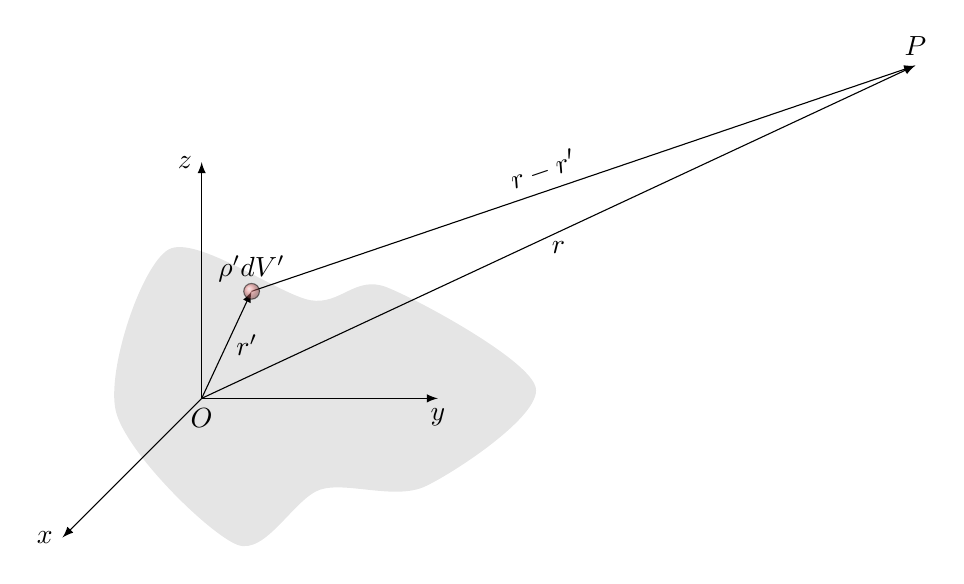
\begin{tikzpicture}
        \pgfmathsetseed{10}
		\fill[gray!20] plot [smooth cycle, samples=8,domain={1:8}] (\x*360/8+6*rnd:1cm+2cm*rnd);
		\coordinate (O) at (-1.5,0);
        \draw[-latex] (O) -- +(3,0) node[below] {$y$};
		\draw[-latex] (O) -- +(0,3) node[left] {$z$};
		\draw[-latex] (O) -- +(225:2.5) node[left] {$x$};
		\node[below] at (O) {$O$};
		\draw[-latex] (O) --  node[pos=0.5, anchor=west] {$\vect{r'}$} +(65:1.5) coordinate (endp);
		\draw[-latex] (O) -- node[pos=0.5, below] {$\vect{r}$} +(25:10) coordinate (end) ;
		\draw[-latex] (endp) -- (end) node[pos=0.45, above, sloped] {$\vect{r} - \vect{r'}$};
		\draw[ball color=red!50, opacity=0.5] (endp) circle (0.1) node[above, opacity=1] {$\rho'dV'$};
		\node[above] at (end) {$P$};
    \end{tikzpicture}
\captionof{figure}{Тіло із заданим розподілом заряду $\rho(\vect{r'})$\label{charge_distribution}}
\end{center}
%---------------------------------------------------------

Потік вектора напруженості електричного поля через довільну поверхню $S$:
\begin{equation}
	\Phi_{\Efield} = \iint\limits_{S}\Efield\cdot d\vect{S}
\end{equation}

Теорема Гауса для вектора напруженості електричного поля: потік вектора напруженості електричного поля через довільну замкнену поверхню $S$ не залежить лише від заряду, що знаходиться всередині цієї поверхні
\begin{equation}\label{GaussLow}
	\oiint\limits_{S}\Efield\cdot d\vect{S} = 4\pi\iiint\limits_{V}\rho dV
\end{equation}
\end{Theory}

%=========================================================
\begin{problem}
    У двох точках на одній лінії з точковим зарядом напруженість електричного поля складає $E_1$ і $E_2$, відповідно. Чому вона дорівнює посередині між цими точками?
\begin{solution}
	$E = \frac{4E_1E_2}{(\sqrt{E_1} + \sqrt{E_2})^2}$.
\end{solution}
\end{problem}

%=========================================================
\begin{problem}
    Напруженість електричного поля в центрі кривизни рівномірно зарядженого півкільця складає $E$. Чому вона дорівнює в центрі кільця такого самого радіуса і з таким самим зарядом?
\end{problem}

%=========================================================
\begin{problem}
    Як вплине на силу взаємодії заряджених кульок у двох вершинах правильного трикутника така сама заряджена кулька, вміщена в третю вершину?
\end{problem}

\subsection*{Задачі на використання принципу суперпозиції}

%=========================================================
\begin{problem}\label{prb:thread}
За допомогою принципу суперпозиції обчисліть напруженість електричного поля в точці, яка розташована на відстані $r$ від тонкої рівномірно зарядженої нитки з густиною заряду $\lambda$.
\begin{solution}
	$E = \frac{2\lambda}{r}.$
\end{solution}
\end{problem}


%=========================================================
%\begin{problem}
%На поверхню нескінченної площини з поверхневим зарядом $\sigma$ нанесено шар матеріалу товщиною $d$, який має рівномірний розподіл заряду густиною~$\rho$. Визначте напруженість електричного поля у всіх точках простору.
%\begin{solution}
%	$E_z =
%		\begin{cases}
%			-2\pi (\sigma + \rho d),                    & x < d    \\
%			2\pi \left( \sigma -\rho (d - 2x) \right) , & 0< x < d \\
%			2\pi (\sigma + \rho d),                     & x > d
%		\end{cases}
%	$
%\end{solution}
%\end{problem}

%=========================================================
\begin{problem}\label{prb:disk}
За допомогою принципу суперпозиції обчисліть напруженість електричного поля в точці, яка розташована на осі тонкого, рівномірно зарядженого диска з густиною заряду $\sigma$ радіусом~$R$, на відстані $z$ від його центру.
\begin{solution}
	$E_z = 2\pi\sigma \left( 1 - \frac{z}{\sqrt{R^2 + z^2}}\right)$
\end{solution}
\end{problem}

%=========================================================
\begin{problem}\label{prb:surface}
Заряд рівномірно розподілений по поверхні нескінченної тонкої пластини з поверхневою густиною заряду $\sigma$. Визначити напруженість електричного поля над поверхнею пластини.
\begin{solution}
	$E_z = 2\pi\sigma$.
\end{solution}
\end{problem}

%=========================================================
\begin{problem}\label{hemisphere}
Заряд рівномірно розподілений по поверхні напівсфери радіуса $R$ з поверхневою густиною заряду $\sigma$. Визначити напруженість електричного поля в центрі напівсфери.
\begin{solution}
	$E_z = \pi\sigma$.
\end{solution}
\end{problem}

%=========================================================
\begin{problem}
Дві однорідно і різнойменно заряджені поверхневою густиною $\sigma$ нескінченні площини перетинаються під прямим кутом. Знайти величину та напрямок напруженості електростатичного поля в довільній точці та побудувати силові лінії.
\begin{solution}
	$E=2\sqrt{2}\pi\sigma$
\end{solution}
\end{problem}

%=========================================================
\begin{problem}
Тонке кільце радіусом $R$ заряджене з лінійною густиною, яка змінюється за законом $\lambda = \lambda_0\cos\phi$, де $\lambda_0$~-- постійна, $\phi$~-- полярний кут. Знайти модуль напруженості електричного
поля:
\begin{enumerate*}[label=\alph*)]
	\item в центрі кільця;
	\item на осі кільця в залежності від відстані $z$ до його
	центру.
\end{enumerate*}
Дослідити отриманий вираз при $z \gg R$.
\begin{solution}
	\begin{enumerate*}[label=\alph*)]
		\item $E = \frac{\pi\lambda_0}{R}$;
		\item $E = \frac{\pi\lambda_0R^2}{\left( z^2 + R^2\right)^{\nfrac{3}{2}}}$.
	\end{enumerate*}
\end{solution}
\end{problem}

%=========================================================
\begin{problem}
    Рівномірно заряджена з поверхневою густиною $\rho$ нескінченна тонка пластина розділена на дві половини щілиною ширини $d$. Знайти напруженість електричного поля на великих відстанях $r \gg d$ від щілини.
\begin{solution}
	$\Efield = 2\pi\sigma\frac{\vect{r}}{r} - 2d\sigma\frac{\vect{r}}{r^2}$, де $\vect{r}$~--- радіус-вектор проведений від осі симетрії щілини в точку спостереження.
\end{solution}
\end{problem}


%=========================================================
\begin{problem}\label{prb:sph}
Сфера радіуса $R$ , яка заряджена з поверхневою густиною заряду $\sigma = \vect{a}\cdot\vect{r}$, де $\vect{a}$~-- постійний вектор, $\vect{r}$~-- радіус-вектор точки сфери відносно її центру (рис.~\ref{sph}). Знайти напруженість $\Efield$ електричного поля в центрі сфери.
\begin{solution}
	$\Efield = \frac43 \pi R \vect{a}$
\end{solution}
\end{problem}
%---------------------------------------------------------
\begin{figure}[h!]\centering
	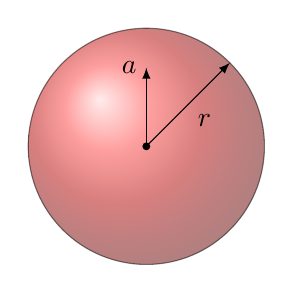
\begin{tikzpicture}
		\draw[ball color=red, opacity=0.5] (0,0) circle (1.5);
		\fill[black] (0,0) circle (0.05);
		\draw[-latex] (0,0) -- (0,1) node[left] {$\vect{a}$};
		\draw[-latex] (0,0) -- node[below right] {$\vect{r}$} (45:1.5);
	\end{tikzpicture}
	\caption{До задачі~\ref{prb:sph}}
	\label{sph}
%---------------------------------------------------------
\end{figure}

%=========================================================
\begin{problem}\label{prb:sphere_on_pane}
На нескінченній площині, що рівномірно заряджена з поверхневою густиною~$\sigma$, лежить оболонка напівсфери, яка торкається площини тільки своїм полюсом (рис.~\ref{sphere_on_pane}). Знайти напруженість електричного поля у центрі основи оболонки, точці $O$, якщо півсфера заряджена з густиною~$-\sigma$.
\begin{solution}
	$E_z = \pi\sigma$.
\end{solution}
\end{problem}

%=========================================================
\begin{problem}\label{prb:hole_in_pane}
У нескінченній тонкій площині, яка заряджена рівномірно з поверхневою густиною заряду $\sigma$, вирізано круглий отвір радіусом $R$ (рис.~\ref{hole_in_pane}). Знайти напруженість електричного поля на осі цього отвору.
\begin{solution}
	$E_z = \frac{2\pi\sigma z}{\sqrt{R^2 + z^2}}$
\end{solution}
\end{problem}

%=========================================================
\begin{figure}[h!]\centering
	%---------------------------------------------------------
	\begin{minipage}[t]{0.45\linewidth}\centering
		%---------------------------------------------------------
		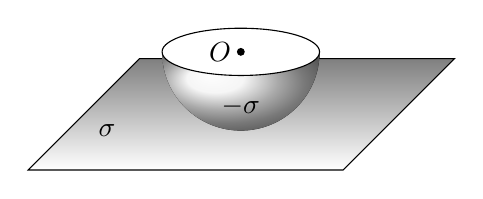
\begin{tikzpicture}
			\shade[red!20, draw=black] (-2,-1) -- ++(4,0) -- ++(45:2) -- +(-4,0) -- cycle;
			\node at (-1,-0.5) {$\sigma$};
			\fill[ball color=gray!10] (-0.3,0.5) arc (-180:0:1) -- cycle;
			\fill[white, draw=black] (0.7,0.5) ellipse (1 and 0.3);
			\fill[black] (0.7,0.5) circle (0.05) node[left] {$O$};
			\node at (0.7,-0.2) {$-\sigma$};
		\end{tikzpicture}
		\caption{До задачі~\ref{prb:sphere_on_pane}}
		\label{sphere_on_pane}
		%---------------------------------------------------------
	\end{minipage}
	%---------------------------------------------------------
	\begin{minipage}[t]{0.45\linewidth}\centering
		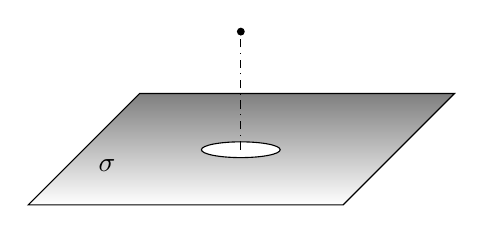
\begin{tikzpicture}
			\shade[red!20, draw=black] (-2,-1) -- ++(4,0) -- ++(45:2) -- +(-4,0) -- cycle;
			\node at (-1,-0.5) {$\sigma$};
			\fill[white, draw=black] (0.7,-0.3) ellipse (0.5 and 0.1);
			\draw[dash dot] (0.7,-0.3) -- ([yshift=1.5cm]0.7,-0.3) coordinate (O);
			\fill (O) circle (0.05) ; %node[left] {$O$};
		\end{tikzpicture}
		\caption{До задачі~\ref{prb:hole_in_pane}}
		\label{hole_in_pane}
	\end{minipage}
	%---------------------------------------------------------
\end{figure}

%=========================================================
\begin{problem}
У сфері, яка заряджена рівномірно з поверхневою густиною заряду $\sigma$, вирізано круглий отвір, малий в порівнянні з радіусом сфери. Знайти напруженість поля в центрі цього отвору.
\begin{solution}
	$E_z = 2\pi\sigma$.
\end{solution}
\end{problem}

%=========================================================
\begin{problem}
У сфері радіусом $R$, яка заряджена рівномірно з поверхневою густиною заряду $\sigma$, вирізано круглий отвір радіусом $r$, малий в порівнянні з радіусом сфери ($r \ll R$). Знайти напруженість поля в центрі сфери.
\begin{solution}
	$\Efield =-\frac{\pi r^2 \sigma}{R^3}\vect{r}$, де $\vect{r}$~--- радіус-вектор з початком у центрі вирізаного отвору і кінцем у центрі сфери.
\end{solution}
\end{problem}

%%=========================================================
%\begin{problem}
%У необмеженому плоскому шарі товщиною $2d$ об'ємна густина заряду змінюється за законом $\rho = \rho_0\frac{x}{d}$, де $x$~--- вісь, перпендикулярна площині шару. В шарі є тонкий
%канал вздовж осі $x$, в якому знаходиться точковий диполь з масою $m$ і дипольним моментом $p$. Визначити період малих поздовжніх коливань диполя.
%\begin{solution}
%	$T = \sqrt{\frac{\pi md}{p\rho_0}}$.
%\end{solution}
%\end{problem}

\subsection*{Визначення потоку електростатичного поля через довільні поверхні}

%=========================================================
\begin{problem}
Поле створюється в вакуумі рівномірно зарядженою прямолінійною нескінченною ниткою. Лінійна густина заряду дорівнює $\lambda$. Обчислити потік вектора напруженості цього поля через поверхню квадрата зі стороною $l$, площина якого паралельна зарядженій нитці і розташована від неї на відстані~$l/2$.
\begin{solution}
	$\Phi = \pi l \lambda$
\end{solution}
\end{problem}

%=========================================================
\begin{problem}
Напівнескінченна рівномірно заряджена нитка має лінійну густину заряду $\lambda$. Знайти потік електричного поля через кільце радіусом $R$, центр якого співпадає з кінцем нитки. Нитка перпендикулярна до площини кільця.
\begin{solution}
	$\Phi = 2\pi\lambda R$.
\end{solution}
\end{problem}

%=========================================================
\begin{problem}
Точковий заряд розташований в одній з вершин куба. Знайти потік електричного поля через куб. Визначити потік через кожну з граней куба.
\begin{solution}
	Потік через куб $\Phi = \frac{\pi}{2}q$. Потік через грані, що сходяться у вершині, в якій розташований заряд $\Phi_1 = \Phi_2 =\Phi_3 = 0$, потік через інші грані $\Phi_4 = \Phi_5 =\Phi_6 = \frac{\pi}{6}q$.
\end{solution}
\end{problem}

%%=========================================================
%\begin{problem}
%Два різнойменних точкових заряди абсолютною величиною $q$ знаходяться на відстані $2l$ один від одного. Знайти потік вектора напруженості електричного поля через поверхню кола радіусом $R$, центр якого розташований на осі, що з'єднує заряди, а його площина перпендикулярна до цієї осі.
%\begin{solution}
%$\Phi = 4\pi q \left( 1 - \frac{l}{\sqrt{R^2 + l^2 }}\right) $.
%\end{solution}
%\end{problem}

%=========================================================
\begin{problem}
Заряд $q$ знаходиться на осі кільця радіусом $R$. Відстань від заряду до центра кільця дорівнює $l$. Знайти потік електричного поля через через поверхню, що охоплюється кільцем.
\begin{solution}
	$\Phi = 2\pi q\left( 1 - \frac{l}{\sqrt{R^2 + l^2}}\right) $.
\end{solution}
\end{problem}

\subsection*{Визначення напруженості електростатичного поля за допомогою теореми Гауса}

%=========================================================
\begin{problem}
	За допомогою теореми Гауса обчисліть напруженість електричного поля в точці, яка розташована на відстані $r$ від
\begin{enumerate*}[label=\alph*)]
\item тонкої рівномірно зарядженої нитки з густиною заряду $\lambda$,
\item нескінченної рівномірно зарядженої площини з густиною заряду $\sigma$.
\end{enumerate*}
\end{problem}

%=========================================================
\begin{problem}
    Знайдіть напруженість електричного поля в середині та зовні нескінченного рівномірно зарядженого циліндра густиною заряду $\rho$ та радіусом $R$. Накресліть графік $E(r)$.
\begin{solution}
	$\Efield =
		\begin{cases}
			2\pi\rho r\\
			\frac{2\pi\rho R^2}{r}.
		\end{cases}
	$
\end{solution}
\end{problem}

%=========================================================
\begin{problem}
    Знайдіть напруженість електричного поля в середині та зовні рівномірно зарядженої сфери густиною заряду $\rho$ та радіусом $R$. Накресліть графік $E(r)$.
\begin{solution}
	$E =
		\begin{cases}
			\rho\frac{4\pi\rho}{3}r\\
			\rho\frac{4\pi\rho R^3}{3 r^2}.
		\end{cases}
	$
\end{solution}
\end{problem}

%=========================================================
\begin{problem}
    Усередині нескінченного циліндра, однорідно зарядженого з об'ємною густиною $\rho$, є циліндрична порожнина. Відстань між паралельними осями циліндра і порожнини одорівнює $l$. Знайти напруженість електричного поля всередині порожнини.
\begin{solution}
	$\Efield = 2\pi\rho \vect{l}$, де $\vect{l}$~--- вектор, проведений від центру циліндра до центру порожнини.
\end{solution}
\end{problem}


%=========================================================
\begin{problem}
Сферична порожнина розташована ексцентрично в середині кулі, яка однорідно зарядженого по об'єму з густиною
$\rho$. Відстань між центрами кулі і порожнини дорівнює $l$. Визначити напруженість $\Efield$ електричного поля в точках порожнини.
\begin{solution}
	$\Efield = \frac{4\pi}{3}\rho \vect{l}$, де $\vect{l}$~--- вектор, проведений від центру кулі до центру порожнини.
\end{solution}
\end{problem}

%=========================================================
\begin{problem}
Система складається з кулі радіусом $R$, яка заряджена рівномірно, і навколишнього середовища, що заповнене зарядом з об'ємною густиною $\rho = \frac{a}{r}$, де $a$~-- константа, $r$~-- відстань до центру кулі. Знайти заряд кулі, при якому модуль вектора напруженості електричного поля поза її межами не буде залежати від $r$.
\begin{solution}
	$q = 2\pi a R^2$
\end{solution}
\end{problem}

%=========================================================
\begin{problem}
Середня густина заряду електронної хмари в атомі водню дорівнює $\rho~=~-\frac{e}{\pi a^3}\exp{\left( -\frac{2r}{a}\right) }$, де $-e$~--- заряд електрона, $a$~-- борівський радіус, а $r$~-- відстань до протона. Визначити напруженість $\Efield$ електричного поля поля в атомі водню. Дослідити $\Efield$ на малих ($r\ll a$) та  великих ($r \gg a$) відстанях від протона.
\begin{solution}
	$\Efield = \frac{e\vect{r}}{r^3} \left[ 1 + \frac{2r}{a} \left( 1 + \frac{r}{a} \right) \right]\exp{\left( -\frac{2r}{a}\right) }$. При $r\ll a$, $\Efield = \frac{e\vect{r}}{r^3}$, при $r \gg a$, $\Efield = \frac{2e\vect{r}}{a^2r}\exp{\left( -\frac{2r}{a}\right) }.$
\end{solution}
\end{problem}

\section{Дипольний момент. Поле диполя. Сили, що діють на диполь з боку поля.}

\begin{Theory}
Електричний дипольний момент системи точкових зарядів:
	\begin{equation}
		\vect{p}_e = \sum\limits_i q_i\vect{r}_i
	\end{equation}
Електричний дипольний момент зарядженого тіла:
	\begin{equation}
	\vect{p} = \iiint\limits_V\rho\vect{r}dV.
	\end{equation}

Напруженість поля електричного диполя:
	\begin{equation}\label{E_dipole}
	\Efield = \frac{3(\vect{p}\cdot\vect{r})\vect{r}}{r^5} - \frac{\vect{p}}{r^3}.
	\end{equation}

%---------------------------------------------------------
\begin{center}
	\begin{tikzpicture}[scale=0.5, every node/.style={transform shape}, rotate=180]
		\clip (-3.5,-8.1) rectangle (3.5,8.1);
		\foreach \i [evaluate=\i as \j using abs(\i)] in {-40,-12,-8,-6,...,8,12,40} {
				\ifnum\i<0\def\domain{1:179}\else\def\domain{179:1}\fi
				%\ifnum\j>12\def\position{0.05}\else\def\position{0.1}\fi
				\draw [color=red,
					samples=200,
					domain=\domain,
					decoration={markings, mark=at position 0.02 with {\arrow{latex'}}},
					decoration={markings, mark=at position 0.1 with {\arrow{latex'}}},
					decoration={markings, mark=at position 0.5 with {\arrow{latex'}}},
					decoration={markings, mark=at position 0.9 with {\arrow{latex'}}},
					decoration={markings, mark=at position 0.98 with {\arrow{latex'}}},
					postaction={decorate}
				] plot (xy polar cs:angle=\x,radius= {\i*(sin(\x))^2});
			}
\draw [color=red, decoration={markings, mark=at position 0.5 with {\arrow{latex'}}},
					postaction={decorate}
				] (4,0) -- (0,0);
\draw [color=red, decoration={markings, mark=at position 0.5 with {\arrow{latex'}}},
					postaction={decorate}
				] (0,0) -- (-4,0);
		\fill[white] (0,0) circle (1);
		\draw[ball color = red!50] (-0.5,0) circle (0.2);\node at (-0.5,0) {$+$};
		\draw[ball color = blue!50] (0.5,0) circle (0.2);\node at (0.5,0) {$-$};
		\draw[latex-] (-0.3,0) -- (0.3,0);
	\end{tikzpicture}
\captionof{figure}{Електричне поле диполя}
\end{center}
%---------------------------------------------------------

Сила, що діє на електричний диполь з боку електричного поля:
	\begin{equation}
		\vect{F} = (\vect{p}\vect{\nabla})\Efield.
	\end{equation}
Момент сили, що діє на диполь в електричному полі:
	\begin{equation}
		\vect{M} = \left[ \vect{p}\times \vect{E}\right].
	\end{equation}
\end{Theory}

%=========================================================
\begin{problem}
    Визначте електричний дипольний момент системи, що складається з двох різнойменних однакових за модулем зарядів. Як напрямлена ця величина? Чи залежить ця величина від вибору початку координат?
\end{problem}


%=========================================================
\begin{problem}\label{prb:semiring}
У центрі півкільця радіусом $R$ знаходиться точковий заряд $-q$. Півкільце має повний заряд $+ q$, розподілений за законом $\lambda\sim\cos\phi $, де $\lambda$~-- лінійна густина заряду, $\phi$~-- кут між радіусом-вектором даної точки і віссю симетрії системи $Oz$ (рис.~\ref{semiring}). В дипольному наближенні знайти напруженість електричного поля на осі $Oz$ на відстані $z$ від системи ($z \gg R$).
\begin{solution}
	$E_z = \frac{\pi qR}{2z^3}$
\end{solution}
\end{problem}

%=========================================================
\begin{problem}\label{prb:volume_of_capacitor}
На відстані $l$ від плоского конденсатора напруженість електричного поля дорівнює $E_1$ (рис.~\ref{volume_of_capacitor}). Поле в середині конденсатора $E_2$. Знайдіть об'єм конденсатора. Відомо, що $l$ набагато більше за відстань між пластинами.
%---------------------------------------------------------
\begin{solution}
	$V = \frac{E_1}{E_2}2\pi l^3$.
\end{solution}
\end{problem}

%=========================================================
\begin{figure}[h!]\centering
	%---------------------------------------------------------
	\begin{minipage}[t]{0.45\linewidth}\centering
		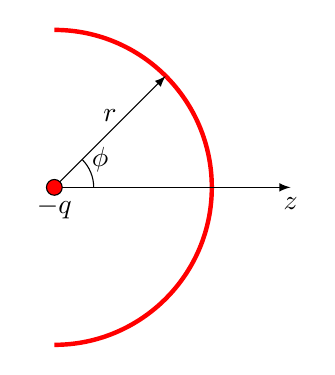
\begin{tikzpicture}
			\draw[red, ultra thick] (0,2) arc (90:-90:2);
			\draw[-latex] (0,0) -- node[above] {$\vect{r}$} (45:2);
			\draw (0.5,0) arc (0:45:0.5) node[right] {$\phi$};
			\draw[-latex] (0,0) -- (3,0) node[below] {$z$};
			\fill[red, draw=black] (0,0) circle (0.1) node[below, black] {$-q$};
		\end{tikzpicture}
		\caption{До задачі~\ref{prb:semiring}}
		\label{semiring}
	\end{minipage}
	%---------------------------------------------------------
	\begin{minipage}[t]{0.45\linewidth}\centering
		\begin{tikzpicture}
			\draw [ultra thick, red] (0,-1) -- (0,1)
			(0.5,-1) -- (0.5,1);
			\draw [dashed] (0.25,0) -- node [below] {$l$} (5,0);
			\fill [black] (5,0) circle (0.05) node [above] {$E_1$};
			\node at (0,-1.85) {}; %comment if alone
		\end{tikzpicture}
		\caption{До задачі~\ref{prb:volume_of_capacitor}}
		\label{volume_of_capacitor}
	\end{minipage}
	%---------------------------------------------------------
\end{figure}

%=========================================================
\begin{problem}\label{dipole-dipole}
Визначити силу взаємодії двох диполей з моментами $\vect{p}_1$ та $\vect{p}_2$, які розміщені на відстані $d$ один від одного і орієнтовані один відносно одного
\begin{enumerate*}[label=\alph*)]
	\item $(\vect{p}_1 \uparrow \uparrow \vect{p}_2) \perp \vect{r}$,
	\item $(\vect{p}_1 \downarrow \uparrow \vect{p}_2) \perp \vect{r}$,
	\item $\vect{p}_1 \uparrow \uparrow \vect{p}_2 \uparrow \vect{r}$,
	\item $\vect{p}_1 \downarrow \uparrow \vect{p}_2 \uparrow \uparrow \vect{r}$,
\end{enumerate*}
де $\vect{r}$~-- радіус-вектор напрямлений від диполя $1$ до диполя $2$.
%---------------------------------------------------------
\begin{solution}
	\begin{enumerate*}[label=\alph*)]
		\item $F = \frac{3 p_1 p_2}{d^4}$, диполі відштовхуються,
		\item $F = \frac{3 p_1 p_2}{d^4}$, диполі притягуються,
		\item $F = \frac{6 p_1 p_2}{d^4}$, диполі притягуються,
		\item $F = \frac{6 p_1 p_2}{d^4}$, диполі відштовхуються.
	\end{enumerate*}
\end{solution}
\end{problem}

%=========================================================
\begin{problem}\label{wire-dipole}
Частинка з дипольним моментом $\vect{p}$ розміщена на відстані $r$ від довгого зарядженого дроту, густина поверхневого заряду на якому $\lambda$. Знайти силу та момент сил взаємодії частинки та дроту, якщо:
\begin{enumerate*}[label=\alph*)]
	\item $\vect{p}$ напрямлений паралельно дроту,
	\item $\vect{p}$ напрямлений перпендикулярно до дроту,
	\item $\vect{p}$ напрямлений перпендикулярно дроту і лежить в паралельній до нього площині.
\end{enumerate*}
\begin{solution}
	Вказівка: Сила, що діє на диполь в неоднорідному магнітному полі визначається за формулою $\vect{F} = (\vect{p}\cdot\nabla)\Efield$, а момент сили $\vect{M} = \left[ \vect{p}\times\Efield\right]  + \left[ \vect{r}\times\vect{F}\right] $.

	\begin{enumerate*}[label=\alph*)]
		\item $\vect{F} = 0$, $\vect{M} = \frac{2\lambda}{r^2} \left[ \vect{p}\times\vect{r}\right] $,
		\item $\vect{F} = \frac{2\lambda \vect{p}}{r^2}$, $\vect{M} = 0$,
		\item $\vect{F} = \frac{2\lambda \vect{p}}{r^2}$, $\vect{M} = 0$.
	\end{enumerate*}
\end{solution}
\end{problem}

%=========================================================
\begin{problem}
    Знайдіть силу і обертовий момент, що діють на диполь $\vect{p}$ в полі точкового заряда $q$.
\end{problem}


%=========================================================
\begin{problem}\label{prb:perp_dipoles}
Два однакові точкові диполі з моментом $p$, розташовано взаємно перпендикулярно на відстані $r$ (рис.~\ref{perp_dipoles}). Які обертові моменти діють на  кожен з диполів та на всю систему в цілому?
\begin{solution}
	$M_1 = -\frac{p^2}{r^3}$, $M_2 = -\frac{2p^2}{r^3}$. Обертовий момент, що діє на систему дорівнює нулю.
\end{solution}
\end{problem}
%---------------------------------------------------------
\begin{figure}[h!]\centering
	\begin{tikzpicture}
		\draw[-latex, red, thick] (-1,0) -- +(0,2) node[left, black] {$\vect{p}_1$};
		\draw[-latex, red, thick] (5,1) -- +(-2,0) node[below, black] {$\vect{p}_2$};;
		\draw[dash dot] (3,1) -- node[below] {$r$} (-1,1);
	\end{tikzpicture}
	\caption{До задачі~\ref{prb:perp_dipoles}}
	\label{perp_dipoles}
\end{figure}
%---------------------------------------------------------

%=========================================================
\begin{problem}%Черкасский
Незаряджена металева куля радіуса $R$ вноситься в електричне поле, яке за відсутності кулі було однорідним і дорівнювало $\Efield_0$. Знайти дипольний момент кулі. Визначити густину поверхневих зарядів на кулі. Знайти повний заряд, індукований на одній половині поверхні кулі.
\begin{solution}
	$\vect{p} = \Efield_0 R^3$,
	$\sigma = \frac{3}{4\pi} \frac{\left( \Efield_0\cdot\vect{r}\right) }{r}$,
	$Q = \frac34 E_0 R^2$
\end{solution}
\end{problem}

%=========================================================
\begin{problem}
З якою силою взаємодіють дві незаряджені кулі радіусами $R$, що вміщені в однорідне електричне поле напруженістю $\Efield_0$, яке напрямлене
\begin{enumerate*}[label=\alph*)]
	\item вздовж прямої, що з'єднує центри куль,
	\item перпендикулярно до прямої, що з'єднує центри куль.
\end{enumerate*}
Відстань між кулями $l \gg R$?
\begin{solution}
	\begin{enumerate*}[label=\alph*)]
		\item $F = \frac{6\Efield_0^2R^6}{l^4}$, кулі притягуються,
		\item $F = \frac{3\Efield_0^2R^6}{l^4}$, кулі відштовхуються.
	\end{enumerate*}
\end{solution}
\end{problem}

\section{Поняття потенціалу. Зв'язок потенціалу і напруженості}

 \begin{Theory}\small
	Робота сил електростатичного поля по переміщенню заряду $q$ з точки $1$ в точку $2$ дорівнює:
	\begin{equation}\label{work}
		A_{12} = q\int\limits_1^2 \vect{E}d\vect{r}.
	\end{equation}

	Робота сил електростатичного поля по переміщенню заряду вздовж замкненого контуру дорівнює нулю, а отже, електростатичне поле є потенціальним полем. Тому роботу можна записати роботу через різницю потенціалів:
	\begin{equation}\label{work_potential}
		A_{12} = q(\phi_1 - \phi_2),
	\end{equation}

	У випадку точкового заряду $Q$, потенціал дорівнює:
	\begin{equation}\label{pot_point}
	\phi = \frac{Q}{r},
	\end{equation}
	де $r$~--- відстань від заряду $Q$ до довільної точки поля.

  Потенціал поля суцільного тіла (принцип суперпозиції):
  \begin{equation}\label{Supperposition_principle}
	  \phi(\vect{r}) = \iiint\limits_{V'} \frac{\rho(\vect{r'}) dV'}{\left| \vect{r} - \vect{r'} \right|}.
  \end{equation}
  де $\vect{r}'$~--- радіус-вектор елементів заряду $\rho(\vect{r'}) dV'$, а $\vect{r}$~--- радіус-вектор точки спостереження.

Потенціал диполя:
	\begin{equation}\label{electric_dipole_potential}
		\phi = \frac{\left( \vect{p}_e\cdot \vect{r}\right) }{r^3}
	\end{equation}

  Зв'язок напруженості та потенціалу:
  \begin{equation}\label{E-phi}
	  \Efield = - \vect{\nabla}\phi.
  \end{equation}
\end{Theory}

%=========================================================
\begin{problem}\label{prb:Dphi}
    Чому дорівнює різниця потенціалів між точками $1$ та $2$ біля пластин ідеального конденсатора (рис.~\ref{Dphi}), що заряджений до напруги $V$?

\end{problem}

%---------------------------------------------------------
\begin{figure}[h!]\centering
		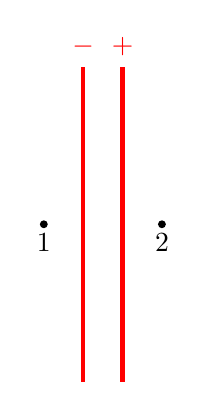
\begin{tikzpicture}
			\draw [ultra thick, red] (0,-2) -- (0,2) node[above] {$-$}
			(0.5,-2) -- (0.5,2) node[above] {$+$};
			\fill (-0.5,0) circle (0.05) node[below, text=black] {$1$};
			\fill (1,0) circle (0.05) node[below, text=black] {$2$};
		\end{tikzpicture}
\caption{До задачі~\ref{prb:Dphi}}
\label{Dphi}
\end{figure}
%---------------------------------------------------------


%=========================================================
\begin{problem}
    Робота сил поля при переміщенні заряду вздовж еквіпотенціальної поверхні $A = 0$. Як це пояснити, адже в кожній точці траєкторії на заряд діє сила $F \neq 0$?

\end{problem}

%=========================================================
\begin{problem}
    У двох точках поля точкового заряду відношення напруженостей $\frac{E_1}{E_2} = \eta$. Чому дорівнює відношення $\frac{\phi_1}{\phi_2}$ потенціалів поля в цих точках?
\begin{solution}
	$\frac{\phi_1}{\phi_2} =\sqrt\eta$.
\end{solution}
\end{problem}

%=========================================================
\begin{problem}
    У двох точках на одній лінії з точковим зарядом потенціал електричного поля дорівнює $\phi_1$ і $\phi_2$, відповідно. Яку величину він має посередині між цими точками?

\end{problem}

%=========================================================
\begin{problem}
    Потенціал електричного поля в центрі зарядженого кільця складає $\phi_0$. Чому він дорівнюватиме, для півкільця такого ж радіусу?
\end{problem}

%=========================================================
\begin{problem}
    Доведіть взаємну ортогональність силових ліній та еквіпотенціальних поверхонь електричного поля.
\end{problem}

%=========================================================
\begin{problem}
    Виведіть формулі зв'язку напруженості та потенціалу~\eqref{E-phi}.
\end{problem}

%=========================================================
\begin{problem}
    Знайдіть вираз для потенціалу, який створюється однорідним електричним полем $\Efield$.
\begin{solution}
	$\phi = -\Efield\cdot\vect{r}$, де $\vect{r}$~-- радіус вектор довільної точки поля.
\end{solution}
\end{problem}

%=========================================================
\begin{problem}
Знайти потенціал тонкого кільця радіусом $R$, яке рівномірно заряджене зарядом $q$ як функцію відстані $r$ від центра кільця при $r \gg R$.
\begin{solution}
	$\phi = \frac{q}{r} + \frac{q}{4r}\left(\frac{R}{r} \right)^2(1-3\cos^2\theta) $
\end{solution}
\end{problem}

%=========================================================
\begin{problem}
Два коаксіальних тонких однорідно заряджених кільця однаковими радіусами $R$ розташовані на відстані $a$, один від одного. Заряди кілець $+q$ і
$-q$ відповідно. Знайти різницю потенціалів між центрами кілець.
\begin{solution}
	$\Delta\phi = \frac{2q}{R}\left(1 - \frac{1}{\sqrt{1 + \left(\frac{a}{R} \right)^2}}\right)$
\end{solution}
\end{problem}

%=========================================================
\begin{problem}
Обчисліть потенціал електричного поля в точці, яка розташована на осі тонкого рівномірно зарядженого диска з густиною заряду $\sigma$ і радіусом $R$, на відстані $z$ від його центру. Знайдіть напруженість електричного поля в цій точці, використовуючи формулу зв'язку напруженості та потенціалу.
\begin{solution}
	$\phi = 2\pi\sigma  \left( \sqrt{R^2 + z^2} - z \right) $.
\end{solution}
\end{problem}

%=========================================================
\begin{problem}
    Знайдіть потенціали для умов задач~\ref{prb:thread} та \ref{prb:surface}.
\end{problem}

%=========================================================
\begin{problem}
    Знайдіть потенціал в середині сфери (в довільній точці), якщо розподіл заряду по поверхні якої задано виразом $\sigma = \vect{a}\cdot\vect{r}$ (див. задачу \ref{prb:sph}).
\begin{solution}
	$\phi = -\frac43\pi R (\vect{a}\cdot\vect{r})$.
\end{solution}
\end{problem}

%=========================================================
\begin{problem}
    За допомогою~\eqref{E-phi} використовуючи ~\eqref{electric_dipole_potential} отримайте формулу для напруженості електричного поля диполя~\eqref{E_dipole}.
\end{problem}


\section{Рівняння Максвелла у випадку електростатики. Рівняння Пуассона та Лапласа}

\begin{Theory}
  Для випадку електростатики у вакуумі, рівняння Максвелла приймають вигляд:
	\begin{align}
		&\oiint\limits_S \Efield\cdot d\vect{S} = 4\pi q  && \text{\small Теорема Гауса для електричного поля} \label{Int I_elstat}\\
		&\oint\limits_L \Efield d\vect{r} =  0 && \text{\small Теорема про циркуляцію для електростатичного поля}\label{Int III_elsta},
	\end{align}
	або у диференціальній формі:
  \begin{align}
	  \divg\Efield & = 4\pi\rho, \label{divE}\\
	  \rot\Efield  & = 0. \label{rotE}
  \end{align}

  З урахуванням зв'язку напруженості та потенціалу~\ref{E-phi}, з рівняння \ref{divE}  отримуємо рівняння Пуассона:
  \begin{equation}\label{Poisson's_equation}
	  \Delta\phi = -4\pi\rho.
  \end{equation}

  В областях, де заряди відсутні, рівняння~\eqref{Poisson's_equation} приймає вигляд:
  \begin{equation}\label{Laplace_equation}
	  \Delta\phi = 0,
  \end{equation}
яке називається рівнянням Лапласа.

Якщо розподіл зарядів в просторі відомий, то розв'язком цих рівнянь буде вираз~\eqref{Supperposition_principle}.
У випадках, якщо в просторі наявні поверхні, на яких потенціали (або його нормальні похідні) відомі, то розв'язок вже не буде простим. Такі задачі називаються задачами з граничними умовами. У випадку заданого розподілу зарядів та заданих граничних умов, розв'язок рівняння Пуассона (або Лапласа) буде мати не більше одного розв'язку, що регламентується теоремою єдиності. Одним із способів розв'язку таких задач, який грунтується на цій теоремі буде розглянуто в \hyperref[image_method]{методі зображень}.
\end{Theory}

%=========================================================
\begin{problem}
    Покажіть, що зв'язок напруженості та потенціалу~\ref{E-phi} сумісний з рівнянням~\ref{rotE}.
\end{problem}


%=========================================================
\begin{problem}
    Розрахуйте $\vect{\nabla}\cdot\vect{r}$ та  $\vect{\nabla}\times\vect{r}$, де $\vect{r}$~--- радіус-вектор довільної точки.
\end{problem}

%=========================================================
\begin{problem}
    Розрахуйте $\vect{\nabla}\cdot\frac{\vect{r}}{r^3}$ та $\vect{\nabla}\times\frac{\vect{r}}{r^3}$, де $\vect{r}$~--- радіус-вектор довільної точки.
\end{problem}

%=========================================================
\begin{problem}
    Розрахуйте $\Delta\frac1r$, де $r$~--- модуль радіус-вектор довільної точки.
\end{problem}

%=========================================================
\begin{problem}
    Густина однорідно зарядженої кулі радіусом $R$ дорівнює $\rho$. Знайдіть $\divg\Efield$ в середині ($r \le R$) та зовні ($r > R$) сфери, де $r$ відстань від центра кулі до довільної точки. Знайдіть напруженість поля в середині та зовні кулі.
\end{problem}

%=========================================================
\begin{problem}
    Чи можна створити в просторі електростатичне поле, напруженість якого виражається формулою $\Efield = \left[ \vect{a}\times\vect{r}\right] $? Зобразіть силові лінії такого поля. Відповідь аргументуйте.
\end{problem}

%=========================================================
\begin{problem}
    Електричне поле однорідне всередині деякої області простору. Чи містять
	внутрішні точки цієї області якісь заряди, які беруть участь у створенні даного електричного поля?
\begin{solution}
	Так. Відповідь обґрунтовується за допомогою теореми Гауса та теореми про циркуляцію.
\end{solution}
\end{problem}

%=========================================================
\begin{problem}
    Доведіть, що якщо потенціал на поверхні деякого порожнього тіла дорівнює $\phi_0$, то в середині провідника він матиме таке ж саме значення.
\end{problem}

%=========================================================
\begin{problem}
    Доведіть на основі рівняння Лапласа, що потенціал в пустому не може мати екстремумів.
\end{problem}

%=========================================================
\begin{problem}
	Доведіть на основі рівняння Лапласа, що середнє значення потенціалу по поверхні довільної сфери дорівнює значенню потенціалу в середині сфери.
\end{problem}

\subsection*{Знаходження значення напруженості чи потенціалу, що створююся заданим розподілом зарядів}

%=========================================================
\begin{problem}
Знайти потенціал  в довільній точці простору
\begin{enumerate*}[label=\alph*)]
	\item сфери радіусом~$R$, рівномірно зарядженої по поверхні густиною заряду~$\sigma$;
	\item кулі радіусом~$R$, рівномірно зарядженої по об'єму густиною заряду~$\rho$;
	\item циліндра радіусом $R$, рівномірно зарядженого лінійною густиною~$\lambda$;
	\item плоского шару товщиною $2a$, рівномірно зарядженого об'ємною густиною~$\rho$.
	\item плоского шару товщиною $2a$, зарядженого об'ємною густиною~$\rho$.
\end{enumerate*}
\begin{solution}
	\begin{enumerate}[label=\alph*)]
		\item $\phi =
		      \begin{cases}
			  \frac{\sigma \pi R^2}{R}, \,    & r < R, \\
			  \frac{\sigma \pi R^2}{r}, \, & r > R
			  \end{cases}
			  $,
		\item $\phi =
			      \begin{cases}
				      \frac23 \pi \rho (3R^2 - r^2), \,    & r < R, \\
				      \frac{4\pi R^3}{3}\frac{\rho}{r}, \, & r > R
			      \end{cases}
		      $,
		\item $\phi =
			      \begin{cases}
				      \lambda \left(1- \frac{r^2}{R^2} \right) ,\, & r < R, \\
				      -2\lambda\ln\frac{r}{R}, \,                  & r > R
			      \end{cases}
		      $,
		\item $\phi =
			      \begin{cases}
				      -2\pi\rho z^2, \,                      & \left| z\right| < a,  \\
				      2\pi\rho a (a - 2\left| z\right| ), \, & \left| z\right| \ge a
			      \end{cases}
		      $
	\end{enumerate}
\end{solution}
\end{problem}

%=========================================================
\begin{problem}
    Знайти потенціал та поле в довільній точці простору плоского шару товщиною $2a$, зарядженого об'ємною густиною~
	\[
		\rho = \begin{cases}
				0, \quad -\infty< x < -a \\
				-\rho_0, \quad -a \le x \le 0, \\
				\rho_0, \quad 0 \le x \le a, \\
				0, \quad a < x < \infty.
				\end{cases}
	\]
	\begin{solution}
		\[
		\phi = \begin{cases}
				0, \quad -\infty< x < -a \\
				2\pi\rho_0 (x+a)^2, \quad -a \le x \le 0, \\
				-2\pi\rho_0 (x-a)^2 + 4\pi\rho_0a^2, \quad 0 \le x \le a, \\
				4\pi\rho_0a^2, \quad a < x < \infty,
				\end{cases}
		\]
		\[
		E = \begin{cases}
				0, \quad -\infty< x < -a \\
				-4\pi\rho_0 (x+a), \quad -a \le x \le 0, \\
				4\pi\rho_0 (x-a), \quad 0 \le x \le a, \\
				0, \quad a < x < \infty,
				\end{cases}
		\]
	\end{solution}
\end{problem}


%=========================================================
\begin{problem}
Кульовий шар між сферами радіусів $R_1$ і $R_2$ ($R_1 < R_2$) заряджений з густиною $\rho = \frac{a}{r^2}$. Знайти потенціал поля в довільній точці.
\begin{solution}
	$
		\phi(r) =
		\begin{cases}
			4\pi a\ln\frac{R_2}{R_1},                                                  & r \le R_1         \\
			4\pi a \left[ \left( 1- \frac{R_1}{r}\right)  + \ln\frac{R_2}{r} \right] , & R_1 \le r \le R_2 \\
			4\pi a \frac{R_2 - R_1}{r},                                                & r \ge R_2
		\end{cases}
	$
\end{solution}
\end{problem}

%=========================================================
\begin{problem}
    Усередині півсфери радіуса $R$ розподілений заряд з об'ємною густиною $\rho = \rho_0e^{ar}$, де $\rho_0$ і $a$~--- додатні постійні, a $r$~--- відстань до центру кривизни півсфери. Знайти напруженість електричного поля в центрі кривизни півсфери.
\begin{solution}
	$E = \frac{\pi\rho_0}{a}(e^{aR} - 1)$.
\end{solution}
\end{problem}


\subsection*{Знаходження розподілу зарядів, що створюють задані значення напруженості чи потенціалу}

%=========================================================
\begin{problem}
Потенціал поля всередині зарядженої кулі залежить тільки від відстані до його центру як $\phi = ar^2 + b$, де $a$ і $b$~-- 	константи. Знайти розподіл об'ємного заряду всередині кулі.
\begin{solution}
	$\rho = \frac{3a}{2\pi}$.
\end{solution}
\end{problem}

%=========================================================
\begin{problem}
Знайти розподіл зарядів, які створюють  потенціал\footnote{Потенціал такого виду називається екранованим кулонівським потенціалом~\cite[\S 1.8, стор.26]{AxiezerGeneralPhysElectro}.} $\phi = \frac{q}{r}e^{-\frac{r}{a}}$, де $a$~--- деяка додатна константа. \emph{Вказівка}: Згадайте, що $\Delta\left(\frac{1}{r}\right) =  -4\pi\delta(r)$, де $\delta(r)$~--- дельта-функція Дірака~\cite[Глава I]{Ivanenko}.
\begin{solution}
	Розподіл зарядів знайдемо з рівняння Пуассона:
	\[
		\Delta\phi = -4\pi\rho.
	\]
	Розпишемо
	\begin{multline*}
		\Delta\phi = \divg\vect{\nabla}\phi = \divg\vect{\nabla}\left( \frac{q}{r}e^{-\frac{r}{a}}\right)  = \\
		= \divg\left( \frac{q}{r}  \vect{\nabla}e^{-\frac{r}{a}} + e^{-\frac{r}{a}}\vect{\nabla}\frac{q}{r}\right) = \\
		= \vect{\nabla}\left( \frac{q}{r}\right) \vect{\nabla}e^{-\frac{r}{a}} + \frac{q}{r}\Delta e^{-\frac{r}{a}} +
		\vect{\nabla}e^{-\frac{r}{a}} \vect{\nabla}\left( \frac{q}{r}\right)  + e^{-\frac{r}{a}}\Delta\left( \frac{q}{r}\right) = \\
		= e^{-\frac{r}{a}}\Delta\left( \frac{q}{r}\right) + 2 \vect{\nabla}\left( \frac{q}{r}\right)\cdot \vect{\nabla}e^{-\frac{r}{a}} + \frac{q}{r}\Delta e^{-\frac{r}{a}} =\\
		= -4\pi q\delta(r)	+ \frac{q}{a^2}\frac{e^{-\frac{r}{a}}}{r}
	\end{multline*}
	Співставляючи останній вираз з рівнянням Пуассона, знайдемо розподіл заряду:
	\[
		\rho = q\delta(r) - \frac{q}{4\pi a^2} \frac{e^{-\frac{r}{a}}}{r},
	\]
	звідки видно, що екранований кулонівський потенціал створюється точковим зарядом, навколо якого розподілена <<хмара>> електричного заряду. Такий характер розподілу зустрічається, наприклад, в електролітах, або плазмі.
\end{solution}
\end{problem}

%=========================================================
\begin{problem}
Напруженість електричного поля в просторі дається формулою:
\[
	\Efield = \frac{e\vect{r}}{r^3}(1 + br)e^{-br}
\]
де $e$ і $b$~-- додатні константи, а $r$~-- відстань до початку координат. Визначити розподіл об'ємної густини заряду, що створює це поле. Чому дорівнює повний заряд $Q$?
\begin{solution}
	$\rho = \frac{eb^2}{4\pi r}e^{-br}$ при $r \neq 0$. $Q = 0$.
\end{solution}
\end{problem}

%=========================================================
\begin{problem}
Заряджена куля радіуса $R$ створює в просторі поле, яке дорівнює $E~=~\frac43\pi\rho_0 r\left( 1- \frac{3r}{4R}\right)$ всередині кулі ($r < R$) і $E = \frac{\pi}{3} \frac{R^3}{r^2}$ зовні ($r > R$). За яким законом розподілено заряд всередині кулі?
\begin{solution}
	$\rho_{\mathrm{in}} = \rho_0\left( 1 - \frac{r}{R}\right)$, при $r <R$, $\rho_{\mathrm{out}} = 0$, при $r > R$.
\end{solution}
\end{problem}

%=========================================================
\begin{problem}
В електронній лампі електрони вилітають із однієї розжареної металевої пластини (катода) і збираються на іншій  плоскій металевій пластині (аноді), яка розташована паралельно на відстані $d$ ($d$ набагато менша за лінійні розміри пластин). Потенціал електричного поля між пластинами змінюється за законом $\phi = kx^{\frac43}$, де $x$~--- відстань від катода. Чому дорівнює густина поверхневих зарядів на пластинах? Як змінюється густина об'ємного заряду $\rho(x)$ в просторі між пластинами?
\begin{solution}
	$\left. \sigma\right|_{x=0} = 0$, $\left. \sigma\right|_{x=d} = -\frac{1}{3\pi}kd^{\frac13}$ , $\rho = -\frac{k}{9\pi} x^{-\frac{2}{3}}$.
\end{solution}
\end{problem}

\section{Провідники в електростатичному полі. Метод електричних зображень}

\begin{Theory}\small
	Основні властивості провідників, вміщених в електростатичне поле:
	\begin{itemize}
		\setlength{\itemsep}{0pt plus 1pt}
		\item Силові лінії електричного поля перпендикулярні до поверхні провідника, отже поверхня провідника в електростатичному полі є еквіпотенціальною поверхнею (\ref{sphere_in_un_mag_field}).
		\item Поле в середині провідника відсутнє $E_{\mathrm{in}} = 0$.
		\item В об'ємі провідника заряди відсутні, заряди розташовуються лише на поверхні провідника.
		\item Поле на поверхні провідника дорівнює $E  = 4\pi\sigma$.
	\end{itemize}

\begin{center}
	\begin{tikzpicture}
	% ============================ параметри ===================================
	\pgfmathsetmacro{\step}{0.4}
	\pgfmathsetmacro{\ea}{5}
	\pgfmathsetmacro{\eb}{1}
	\pgfmathsetmacro{\shape}{1}
	% ============================== функція ===================================
	\draw [
	raw gnuplot, red,
	] plot[id=curve, raw gnuplot] function {
		set isosamples 55, 55;
		set contour base;
		set cntrparam levels incremental -2.2,\step,2.2;
		%set style data lines;
		unset  surface;
		splot [-4:4] [-2.2:2.2] (y*(1+\shape/(x**2 + y**2))) ;
	};
	% ================================ куля ======================================
	\draw[ball color =red!50] (0,0) circle (1.01);
	\node at (0,0) {$E_\mathrm{in} = 0$};
	% ======================= стрілки на лініях ==================================
	\foreach \i in {-2.2,-1.8,...,2.2} {
		\draw[red, -latex', rotate around = {{-asin(\i/(3 +\shape/3))}:({asin(\i/(3 +\shape/3))}:3)}] ({asin(\i/(3 +\shape/3))}:3) -- ({asin(\i/(3 +\shape/3))}:3.1);
		\draw[red, -latex',rotate around = {{180-asin(\i/(3 +\shape/3))}:({180+asin(\i/(3 +\shape/3))}:3)} ] ({180+asin(\i/(3 +\shape/3))}:3) -- ({180+asin(\i/(3 +\shape/3))}:3.1);
	}
	% ============================ знаки зарядів =================================
	\foreach \i in {70,30,15,0}{
		%==================================
		\node at (\i:1.1) {\tiny $+$};
		\node at (-\i:1.1) {\tiny $+$};
		\node at ({180-\i}:1.1) {\tiny $-$};
		\node at ({180+\i}:1.1) {\tiny $-$};
	}
	\end{tikzpicture}
	\captionof{figure}{Металева сфера вміщена в однорідне електричне поле.}
	\label{sphere_in_un_mag_field}
\end{center}
\end{Theory}

\subsection*{Принципові питання електростатики металів}


%=========================================================
\begin{problem}
	Доведіть, що поверхня металу в зовнішньому електростатичному полі є еквіпотенціальною поверхнею.
\end{problem}

%=========================================================
\begin{problem}
	Доведіть, що в присутності зовнішніх електростатичних полів, електричне поле в товщі металу дорівнюватиме нулю. Як змінюватиметься потенціал в просторі в середині металу? На основі теореми Гауса покажіть, що заряд у товщі провідника дорівнюватиме нулю.
\end{problem}

%=========================================================
\begin{problem}
	Доведіть, що електричне поле на поверхні провідника визначається формулою:
	\[
		E = 4\pi\sigma,
	\]
	\noindent де $\sigma$~--- густина поверхневих зарядів на провіднику.
\end{problem}

%=========================================================
%\begin{problem}
%    Максимальна напруженість електричного поля, яке може існувати на поверхні провідника, що межує з вакуумом, за порядком величини дорівнює $10^3$~статВ/см. Вважаючи, що поверхневий заряд, що створює це поле, від'ємний, порівняйте, надлишок електронів з числом атомів, що припадають на ту ж площу.
%\begin{solution}
%
%\end{solution}
%\end{problem}


%=========================================================
\begin{problem}
	Замкнені металеві оболонки мають дві поверхні, зовнішню та внутрішню. Доведіть, що в присутності зовнішніх електростатичних полів, заряди можуть накопичуватись лише на зовнішніх поверхнях металу. (\textit{Вказівка}: Скористайтесь теоремою Гауса та теоремою про циркуляцію для вектора $\vect{E}$.) Яким буде потенціал в порожнині?
\end{problem}


%=========================================================
\begin{problem}
	Доведіть, що при вміщенні електричного заряду $q$ в порожнину незарядженої металевої оболонки, заряд на її внутрішній поверхні дорівнюватиме величині $-q$, а на зовнішній $q$. Чи залежатиме зовнішнє електростатичне поле від положення заряду в середині порожнини? Яким буде заряд внутрішньої та зовнішньої поверхонь порожнини, якщо металева оболонка має заряд $Q$?
\end{problem}



\subsection*{Обчислення потенціалу та напруженості провідника в присутності інших заряджених тіл}


%=========================================================
\begin{problem}\label{potential_of_sphere_in_particle_field}
	Показати, що незаряджена сфера радіусом $R$ вміщена в поле точкового заряду $q$, який знаходиться на відстані $l$ ($l > R$) від її центру матиме потенціал
	\[
		\phi = \frac{q}{l}.
	\]
	Як зміниться потенціал, якщо сфера матиме заряд $Q$?
	\begin{solution}
		$\phi = \frac{q}{l} + \frac{Q}{R}.$
	\end{solution}
\end{problem}


%=========================================================
\begin{problem}
	Показати, що потенціал сфери радіусом $R$, в середину якої вміщено точковий заряд $q$, що знаходиться на відстані $l$ ($l <R$) від її центру не залежатиме від $l$ і дорівнюватиме
	\[
	\phi = \frac{q}{R}.
	\]
	Як зміниться потенціал, якщо сфера матиме заряд $Q$?
	\begin{solution}
		$\phi = \frac{q}{R} + \frac{Q}{R}.$
	\end{solution}
\end{problem}

%=========================================================
\begin{problem}\label{connecting_spheres}
Дві віддалені одна від одної провідні кулі, радіуси яких $R_1$ і $R_2$, несуть заряди $Q_1$ і $Q_2$ відповідно. Чому дорівнюватимуть потенціали і заряди куль після того, як їх з'єднають дротом?
\begin{solution}
	$\phi_1 = \phi_2 = \frac{Q_1 + Q_2}{R_1 + R_2}$, $q_1 = (Q_1 + Q_2) \frac{R_1}{R_1 + R_2}$, $q_2 = (Q_1 + Q_2) \frac{R_2}{R_1 + R_2}$,
\end{solution}
\end{problem}

%=========================================================
\begin{problem}
Металева куля радіусом $R_1$ оточена тонкою металевою концентричною оболонкою радіусом $R_2$, а в простір між ними на відстані $R$ від центру знаходиться точковий заряд $Q$ ($R_1 <R <R_2$). Знайти заряди кулі та оболонки, якщо обидва провідники заземлені?
\begin{solution}
	$q_1 = -Q\frac{R_2-R}{R_2-R_1}\frac{R_1}{R}$, $q_2 = -Q\frac{R-R_1}{R_2-R_1}\frac{R_2}{R}$
\end{solution}
\end{problem}

%=========================================================
\begin{problem}
Дві концентричні сфери з радіусами $R_1$ і $R_2$ ($R_1 < R_2$) отримали заряди $q_1$ і $q_2$ відповідно, які розподілилися рівномірно по їх поверхнях. Знайти потенціал поля в довільній точці на відстані $r$ від центру сфер.
\begin{solution}
	$
		\phi(r) =
		\begin{cases}
			\frac{q_1}{R_1} + \frac{q_2}{R_2}, & r \le R_1         \\
			\frac{q_2}{R_2} + \frac{q_1}{r} ,  & R_1 \le r \le R_2 \\
			\frac{q_1 + q_2}{r} ,              & r \ge R_2
		\end{cases}
	$
\end{solution}
\end{problem}

%=========================================================
\begin{problem}
Точковий заряд $q$ знаходиться на відстані $r$ від центра незарядженого сферичного шару провідника, внутрішній і зовнішній радіуси якого дорівнюють відповідно $R_1$ і $R_2$. Знайти потенціал в центрі сферичного шару, якщо $r < R_1$.
\begin{solution}
	$\phi = q\left( \frac{1}{r} - \frac{1}{R_1} + \frac{1}{R_2}\right) $
\end{solution}
\end{problem}


%=========================================================
\begin{problem}\label{prb:3spheres_middle_ground}
Три концентричні сфери мають радіуси $R_1$, $R_2$ та $R_3$ ($R_1 <R_2 < R_3$). Сфери $1$ та $3$ несуть заряди відповідно $+Q$
і $-Q$. Середня сфера $2$ заземлена провідником (рис.~\ref{3spheres_middle_ground}). Знайти заряд $q$ заземленої сфери $2$ та залежності $E(r)$ та $\phi(r)$ і побудувати їх графіки.
\begin{solution}
	$q=Q\left( \frac{R_2}{R_3} - 1\right) $
\end{solution}
\end{problem}

%=========================================================
\begin{problem}\label{prb:3spheres}
Три концентричні сфери мають радіуси $R_1$, $R_2$ та $R_3$ ($R_1 <R_2 < R_3$). Сфері $2$ надають заряд $+Q$, а сфери $1$ та $3$ з'єднують провідником (рис.~\ref{3spheres}). Знайти заряди сфер $1$ та $3$. Знайти залежності $E(r)$ та $\phi(r)$ і побудувати їх графіки.
\begin{solution}
	$q_1 = - Q\frac{R_3 - R_2}{R_3 - R_1}\cdot \frac{R_1}{R_2}$, $q_2= -q_1$,
	$
		E(r) =
		\begin{cases}
			0,                 & r < R_1       \\
			\frac{q_1}{r^2},   & R_1 < r < R_2 \\
			\frac{Q+q_1}{r^2}, & R_2 < r < R_3 \\
			\frac{Q}{r^2},     & r > R_3
		\end{cases}
	$,

	$
		\phi(r)~=~%
		\begin{cases}
			\frac{q_1}{R_1} + \frac{Q}{R_2} - \frac{q_1}{R_3}, & r < R_1       \\
			\frac{q_1}{r} + \frac{Q}{R_2} - \frac{q_1}{R_3},   & R_1 < r < R_2 \\
			\frac{Q+q_1}{r},                                   & R_2 < r < R_3 \\
			\frac{Q}{r},                                       & r > R_3
		\end{cases}
	$.
\end{solution}
\end{problem}

%=========================================================
\begin{figure}[hb!]\centering
	%---------------------------------------------------------
	\begin{minipage}[b]{0.45\linewidth}\centering
		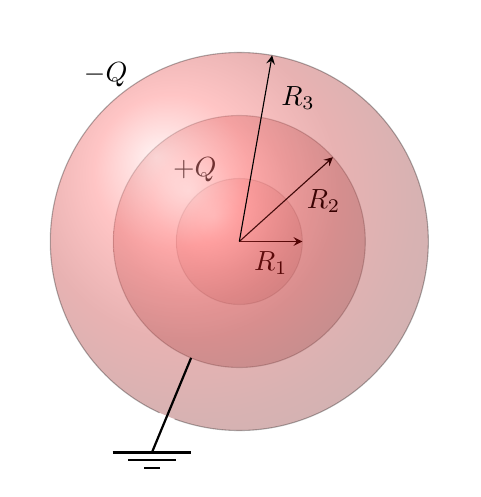
\begin{tikzpicture}
			\def\R{0.8}
			\draw [ball color=red, opacity=0.1] (0,0) circle (\R);
			\draw [-stealth] (0,0) -- node[below] {$R_1$} (0:\R);
			\node [above=2pt] at (135:\R) {$+Q$};
			\draw [ball color=red, opacity=0.2] (0,0) circle ({2*\R});
			\draw [-stealth](0,0) -- node[pos=0.9, below = 5pt] {$R_2$} (42:{2*\R});
			\draw [ball color=red, opacity=0.3] (250:{3*\R}) arc (250:605:{3*\R});
			\draw [-stealth](0,0) -- node[pos=0.9, below right=1pt] {$R_3$} (80:{3*\R});
			\node [above=4pt] at (135:{3*\R}) {$-Q$};
			\draw [thick] (247.5:{2*\R}) -- (247.5:{3*\R +0.5}) coordinate (G);
			\draw [thick] (G) +(-0.5,0) -- +(0.5,0)
			+(-0.3,-0.1) -- +(0.3,-0.1)
			+(-0.1,-0.2) -- +(0.1,-0.2);
		\end{tikzpicture}
		\caption{До задачі~\ref{prb:3spheres_middle_ground}}
		\label{3spheres_middle_ground}
	\end{minipage}
	%---------------------------------------------------------
	\begin{minipage}[b]{0.45\linewidth}\centering
		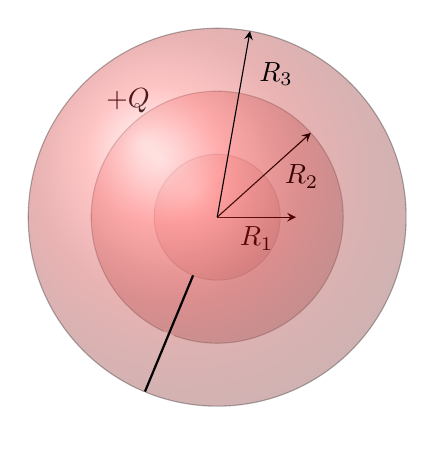
\begin{tikzpicture}
			\def\R{0.8}
			\draw [ball color=red, opacity=0.1] (0,0) circle (\R);
			\draw [-stealth] (0,0) -- node[below] {$R_1$} (0:1);
			\node [above=2pt] at (135:{2*\R}) {$+Q$};
			\draw [ball color=red, opacity=0.2] (250:{2*\R}) arc (250:605:{2*\R});
			\draw [-stealth](0,0) -- node[pos=0.9, below = 5pt] {$R_2$} (42:{2*\R});
			\draw [ball color=red, opacity=0.3] (0,0) circle ({3*\R});
			\draw [-stealth](0,0) -- node[pos=0.9, below right=1pt] {$R_3$} (80:{3*\R});
			\draw[thick] (247.5:\R) -- (247.5:{3*\R});
			\draw[white] (247.5:{3*\R}) -- (247.5:{3*\R+0.7}); % comment when alone
		\end{tikzpicture}
		\caption{До задачі~\ref{prb:3spheres}}
		\label{3spheres}
	\end{minipage}
	%---------------------------------------------------------
\end{figure}

%=========================================================
\begin{problem}\label{prb:3spheres_and_ground}
Розв'язати задачу~\ref{prb:3spheres} за умови, що сферу $3$ заземлюють. Знайти залежності $E(r)$ та $\phi(r)$ і побудувати їх графіки.
\begin{solution}
	$q_1 = -Q\frac{R_1(R_3 - R_2)}{R_2(R_3 - R_1)}$, $q_2 = Q\frac{R_3(R_2 - R_1)}{R_2(R_3 - R_1)}$.
\end{solution}
\end{problem}

%=========================================================
\begin{problem}\label{prb:potential_6_2013-030-036_1}
    У просторі між обкладками незаміщений плоский конденсатор вносять металеву пластину, що має заряд $Q$, так що між пластиною і обкладками конденсатора залишаються зазори $d_1$ та $d_2$ (рис.~\ref{potential_6_2013-030-036_1}). Площі пластини і обкладок конденсатора однакові і дорівнюють $S$. Визначити різницю потенціалів між обкладинками конденсатора. Крайовими ефектами нехтувати.
\begin{solution}
	$\Delta\phi = \frac{2\pi Q}{S} (d_2 - d_1)$.
\end{solution}
\end{problem}

%=========================================================
\begin{problem}
	Обкладки плоского конденсатора, які знаходяться відстані $d = 1$~см. (між ними повітря) заряджаються до напруги $v = 200$~В. Після від'єднання від джерела напруги в конденсатор вміщують пластину з діелектрика товщиною $5$~мм і
	діелектричною проникністю $\epsilon = 2$. Визначити напруженість електричного поля в повітряному зазорі та у вміщеному діелектрику. Яка напруга на конденсаторі після вміщення пластини?
\end{problem}

%=========================================================
\begin{problem}\label{prb:potential_6_2013-030-036_4}
    У плоскому конденсаторі на ліву обкладку поміщають заряд $+Q_1$, а на праву $+Q_2$. Всередину конденсатора паралельно обкладкам поміщають незаряджену металеву пластину (рис.~\ref{potential_6_2013-030-036_1}). Які заряди будуть індуковані на лівій і правій поверхнях пластини, якщо $Q_2>Q_1$?
\begin{solution}
	$Q_{L} = \frac{Q_2 - Q_1}{2}$, $Q_{R} = -Q_{L}$.
\end{solution}
\end{problem}

%=========================================================
\begin{figure}[h!]\centering
%---------------------------------------------------------
\begin{minipage}[t]{0.45\linewidth}\centering
	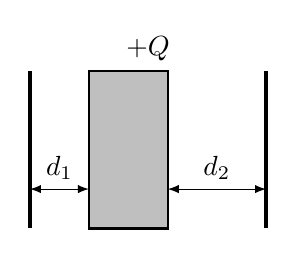
\begin{tikzpicture}
		\draw[ultra thick] (0,0) -- +(0,2);
		\draw[ultra thick] (3,0) -- +(0,2);
		\draw[fill=gray!50, thick] (0.75,0) rectangle (1.75,2) ;
		\node[above] at (1.5,2) {$+Q$};
		\draw[latex-latex] (0,0.5) --node[above] {$d_1$} +(0.75,0);
		\draw[latex-latex] (1.75,0.5) --node[above] {$d_2$} +(1.25,0);
	\end{tikzpicture}
\caption{До задачі~\ref{prb:potential_6_2013-030-036_1}}
\label{potential_6_2013-030-036_1}
\end{minipage}
%---------------------------------------------------------
\begin{minipage}[t]{0.45\linewidth}\centering
	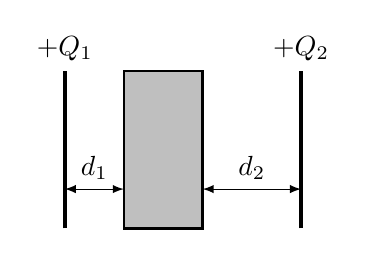
\begin{tikzpicture}
		\draw[ultra thick] (0,0) -- +(0,2);
		\draw[ultra thick] (3,0) -- +(0,2);
		\draw[fill=gray!50, thick] (0.75,0) rectangle (1.75,2) ;
		\node[above] at (0,2) {$+Q_1$};
		\node[above] at (3,2) {$+Q_2$};
		\draw[latex-latex] (0,0.5) --node[above] {$d_1$} +(0.75,0);
		\draw[latex-latex] (1.75,0.5) --node[above] {$d_2$} +(1.25,0);
	\end{tikzpicture}
\caption{До задачі~\ref{prb:potential_6_2013-030-036_4}}
\label{potential_6_2013-030-036_4}
\end{minipage}
%---------------------------------------------------------
\end{figure}
%=========================================================


%=========================================================
\begin{problem}\label{prb:potential_6_2013-030-036_2}
    Три однакові нерухомі металеві пластини розташовані в повітрі на відстані $d_1$ і $d_2$ ($d_2> d_1$) одна від одної. Площа кожної з пластин дорівнює $S$ (рис.~\ref{potential_6_2013-030-036_2}). На середню пластину поміщають позитивний заряд $Q$. Пластини $1$ і $3$ не заряджені і підключені через ключ до резистору з невідомим опором, відмінним від нуля. Які заряди встановляться на пластинах $1$ і $3$ після замикання ключа, через довгий проміжок часу? Крайовими ефектами нехтувати.
\begin{solution}
	$Q_1 = -\frac{Q}{2}\frac{d_2 - d_1}{d_2 + d_1}$, $Q_2 = - Q_1$.
\end{solution}
\end{problem}

%=========================================================
\begin{problem}\label{prb:potential_6_2013-030-036_5}
    Три однакові металеві пластини розташовані в повітрі на однакових відстанях $d$ одна від одної. Площа кожної пластини дорівнює $S$ (рис.~\ref{potential_6_2013-030-036_5}). На пластині $1$ знаходиться позитивний заряд $+Q$. Пластини $2$ і $3$ не заряджені і підключені через ключ до резистору з невідомим відмінним від нуля опором. Які заряди встановляться на пластинах $2$ і $3$ після великого часу після замикання ключа?
\begin{solution}
	$Q_2 = -\frac{Q}{2}$, $Q_3 = \frac{Q}{2}$.
\end{solution}
\end{problem}

%=========================================================
\begin{figure}[h!]\centering
%---------------------------------------------------------
\begin{minipage}[t]{0.45\linewidth}\centering
	\begin{tikzpicture}
		\draw[ultra thick] (0,0) -- +(0,2) node[above] {$1$};
		\draw[ultra thick] (1,0) -- node[pos=0.8, right] {$+Q$} +(0,2) node[above] {$2$};
		\draw[ultra thick] (3,0) -- +(0,2) node[above] {$3$};
		\draw[latex-latex] (0,0.5) --node[above] {$d_1$} +(1,0);
		\draw[latex-latex] (1,0.5) --node[above] {$d_2$} +(2 ,0);
		\draw (0,1) -- ++(-0.5,0) -- ++(0,-2) to[make contact] ++(1,0) to [resistor] ++(3,0) -- ++(0,2) -- ++(-0.5,0);
	\end{tikzpicture}
\caption{До задачі~\ref{prb:potential_6_2013-030-036_2}}
\label{potential_6_2013-030-036_2}
\end{minipage}
%---------------------------------------------------------
\begin{minipage}[t]{0.45\linewidth}\centering
	\begin{tikzpicture}
		\draw[ultra thick] (0,0) -- node[left] {$+Q$}+(0,2) node[above] {$1$};
		\draw[ultra thick] (1,0) -- +(0,2) node[above] {$2$};
		\draw[ultra thick] (2,0) -- +(0,2) node[above] {$3$};
		\draw[latex-latex] (0,0.5) --node[above] {$d$} +(1,0);
		\draw[latex-latex] (1,0.5) --node[above] {$d$} +(1 ,0);
		\draw (1,0) -- ++(0,-0.25) -- ++(-1.5,0) -- ++(0,-0.75) to[make contact] ++(1,0) to [resistor] ++(2,0) -- ++(0,2) -- ++(-0.5,0);
	\end{tikzpicture}
\caption{До задачі~\ref{prb:potential_6_2013-030-036_5}}
\label{potential_6_2013-030-036_5}
\end{minipage}
%---------------------------------------------------------
\end{figure}
%=========================================================

%=========================================================
\begin{problem}\label{prb:potential_6_2013-030-036_3}
    Три тонкі незаряджені металеві пластини площею $S$ кожна розташовані на відстанях $d$ одна від одної, причому $d$ багато менше розмірів пластин. До пластин $2$ і $3$ під'єднали батарею з ЕРС $\EMF$ (рис.~\ref{potential_6_2013-030-036_3}). Пластині $1$ надали позитивний заряд $q_0$. Визначити заряд, який встановився на пластинах $2$ і $3$.
\begin{solution}
	$Q_2 = -\frac{q_0}{2} -\frac{\EMF S}{4\pi d}$, $Q_3 = \frac{q_0}{2} + \frac{\EMF S}{4\pi d}$.
\end{solution}
\end{problem}

%=========================================================
\begin{problem}\label{prb:potential_6_2013-030-036_6}
    Три однакові нерухомі металеві пластини розташовані в повітрі на різних відстанях $d_1$ і $d_2$ ($d_2> d_1$) один від одного (рис.~\ref{potential_6_2013-030-036_6}). На середній пластині $2$ знаходиться позитивний заряд $Q$. Спочатку не заряджені пластини $1$ і $3$ підключають через ключ до батареї з ЕРС $\EMF$. Визначити, які заряди встановилися на пластинах $1$ та $3$ після замикання ключа.
\begin{solution}
	$Q_1 = -\frac{2\EMF S + 4\pi Q(d_2 - d_1)}{8\pi(d_1 + d_2)}$, $Q_3 = -Q_1$.
\end{solution}
\end{problem}
%=========================================================
\begin{figure}[h!]\centering
%---------------------------------------------------------
\begin{minipage}[t]{0.45\linewidth}\centering
	\begin{tikzpicture}
		\draw[ultra thick] (0,0) -- node[left] {$q_0$}+(0,2) node[above] {$1$};
		\draw[ultra thick] (1,0) -- +(0,2) node[above] {$2$};
		\draw[ultra thick] (2,0) -- +(0,2) node[above] {$3$};
		\draw[latex-latex] (0,0.5) --node[above] {$d$} +(1,0);
		\draw[latex-latex] (1,0.5) --node[above] {$d$} +(1 ,0);
		\draw (1,0) -- ++(0,-1) to [battery={info'={$\EMF$},rotate=180}] ++(2,0) -- ++(0,2) -- ++(-1,0);
	\end{tikzpicture}
\caption{До задачі~\ref{prb:potential_6_2013-030-036_3}}
\label{potential_6_2013-030-036_3}
\end{minipage}
%---------------------------------------------------------
\begin{minipage}[t]{0.45\linewidth}\centering
	\begin{tikzpicture}
		\draw[ultra thick] (0,0) -- +(0,2) node[above] {$1$};
		\draw[ultra thick] (1,0) -- node[pos=0.8, right] {$+Q$} +(0,2) node[above] {$2$};
		\draw[ultra thick] (3,0) -- +(0,2) node[above] {$3$};
		\draw[latex-latex] (0,0.5) --node[above] {$d_1$} +(1,0);
		\draw[latex-latex] (1,0.5) --node[above] {$d_2$} +(2 ,0);
		\draw (0,1) -- ++(-0.5,0) -- ++(0,-2) to[make contact] ++(1,0) to [battery={info'={$\EMF$}, rotate=180}] ++(3,0) -- ++(0,2) -- ++(-0.5,0);
	\end{tikzpicture}
\caption{До задачі~\ref{prb:potential_6_2013-030-036_6}}
\label{potential_6_2013-030-036_6}
\end{minipage}
%---------------------------------------------------------
\end{figure}
%=========================================================

\subsection*{Метод зображень. Розподіл зарядів на провідниках, які знаходяться в електричному полі.}\label{image_method}

\begin{Theory}\small

Теорема єдиності в електростатиці обґрунтовує <<метод зображень>>, який допомагає розв'язувати задачі за участю точкового заряду і площині (або декількох площин), точкового заряду і сфери (заземленою і незаземленої) і в ряді інших випадків.
%Задача на метод зображення полягає в наступному: є замкнута область простору з заданими розподілом зарядів і граничними умовами (потенціал на провіднику) і потрібно знайти потенціал (а, отже, і напруженість) в цій області.

Розв'язок задач <<методом зображень>> полягає в підборі фіктивних зарядів поза розглянутою областю, таких, що їх спільне з реальними зарядами поле забезпечує задані граничні умови (потенціал на провіднику). Оскільки всередині області заряди не змінилися, знайдене поле задовольняє рівнянням Пуассона (є його розв'язком). Виконуються також граничні умови. По теоремі єдиності інших рішень немає.


Основні формули методу електричних зображень для сферичних провідників:

\begin{itemize}
	\item для заряду, що знаходиться поза межами заземленої незарядженої сфери, величина заряду-зображення дорівнює:
	\begin{equation}\label{mirror_q_outside}
		q' = -\frac{R}{b}q
	\end{equation}

	\item відстань заряду зображення до центру сфери:
	\begin{equation}\label{mirror_q_outside}
	a = \frac{R^2}{b}
	\end{equation}
\end{itemize}

\begin{center}
	\begin{minipage}[b]{0.45\linewidth}\centering
		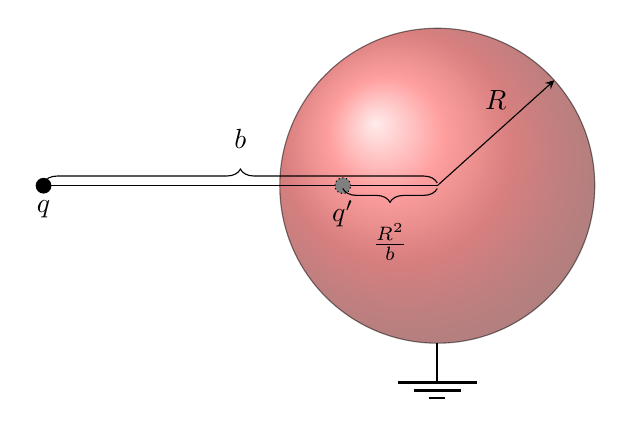
\begin{tikzpicture}
		\def\R{2}
		\fill ({-2.5*\R},0) coordinate (Q) circle (0.1) node[below=2pt] {$q$};
		\draw [ball color=red, opacity=0.5] (0,0) circle (\R);
		\draw [-stealth](0,0) -- node[pos=0.5, above = 5pt] {$R$} (42:2);
		\draw (Q) -- (0,0);
		\draw [densely dotted, fill=gray] ({-0.6*\R},0) coordinate (Qs) circle (0.1) node[below=2pt] {$q'$};
		\draw [decorate, decoration={brace,amplitude=5pt,raise=1pt, mirror}] (0,0) -- node [above=10pt] {$b$} (Q);
		\draw [decorate, decoration={brace,amplitude=5pt,raise=1pt}] (0,0) -- node [below=10pt] {$\frac{R^2}{b}$} (Qs);
		\draw [thick] (0,0) +(-90:\R) -- (-90:{\R+0.5}) coordinate (G);
		\draw [thick] (G) +(-0.5,0) -- +(0.5,0)
		+(-0.3,-0.1) -- +(0.3,-0.1)
		+(-0.1,-0.2) -- +(0.1,-0.2);
		\end{tikzpicture}
		\captionof{figure}{Зображення заряду розміщеного поза незарядженою заземленою сферою\label{image_inside}}
	\end{minipage}
	%---------------------------------------------------------
	\begin{minipage}[b]{0.45\linewidth}\centering
		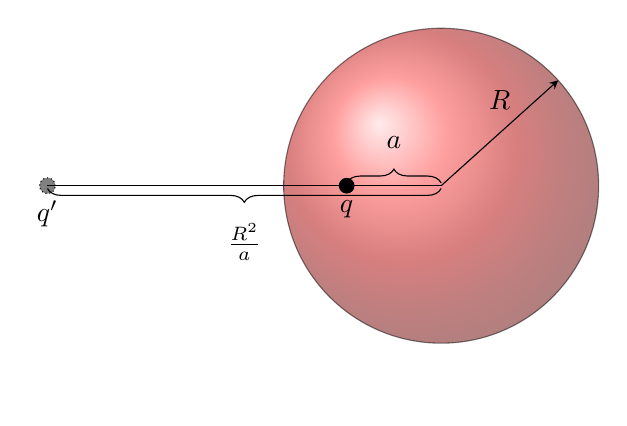
\begin{tikzpicture}
		\def\R{2}
		\draw [densely dotted, fill=gray]  ({-2.5*\R},0) coordinate (Qs) circle (0.1) node[below=2pt] {$q'$};
		\draw [ball color=red, opacity=0.5] (0,0) circle (\R);
		\draw [-stealth](0,0) -- node[pos=0.5, above = 5pt] {$R$} (42:2);
		\draw (Qs) -- (0,0);
		\fill ({-0.6*\R},0) coordinate (Q) circle (0.1) node[below=2pt] {$q$};
		\draw [decorate, decoration={brace,amplitude=5pt,raise=1pt, mirror}] (0,0) -- node [above=10pt] {$a$} (Q);
		\draw [decorate, decoration={brace,amplitude=5pt,raise=1pt}] (0,0) -- node [below=10pt] {$\frac{R^2}{a}$} (Qs);
		\path [thick] (0,0) +(-90:\R) -- (-90:{\R+0.5}) coordinate (G);
		\path [thick] (G) +(-0.5,0) -- +(0.5,0)
		+(-0.3,-0.1) -- +(0.3,-0.1)
		+(-0.1,-0.2) -- +(0.1,-0.2);
		\end{tikzpicture}
		\captionof{figure}{Зображення заряду розміщеного в середині незарядженої сфери\label{image_outside}}
	\end{minipage}
\end{center}
\end{Theory}

%=========================================================
\begin{problem}
    Який заряд наводиться на металевій кулі для випадків, зображених на
	\begin{enumerate*}[label=\alph*)]
	\item  рис.~\ref{image_inside}
	\item  рис.~\ref{image_outside}?
	\end{enumerate*}
\begin{solution}
	\begin{enumerate*}[label=\alph*)]
	\item  $q'$,
	\item  $-q$.
	\end{enumerate*}
\end{solution}
\end{problem}

%=========================================================
\begin{problem}
    Точковий заряд $q$ підноситься на відстань $l$ до центру незаземленої нейтральної металевої кулі радіусом $R$ ($l > R$). Чому дорівнюватиме потенціал кулі? Розв'яжіть задачу методом зображень. Результат порівняйте з задачею~\ref{potential_of_sphere_in_particle_field}. Знайдіть дипольний момент кулі.
	\begin{solution}
		$p = \frac{R^3}{l^2} q$.
	\end{solution}
\end{problem}

%=========================================================
\begin{problem}\label{prb:charge_in_hole}
В металевій ізольованій кулі радіусом $R$ є сферична порожнина, в центрі якої знаходиться заряд $q_0$. Поза кулею на відстані $b$ від її центру розташовано другий заряд $q$ (рис.~\ref{charge_in_hole}). Знайти силу, яка діє на заряд $q$.
\begin{solution}
	$ F =  \frac{qq_0}{b^2} + \frac{q^2 R}{b^3} - \frac{q^2 Rb}{(b^2 - R^2)^2}$.
\end{solution}
\end{problem}

%=========================================================
\begin{problem}\label{prb:charges_in_holes}
В металевій кулі радіусом $R$ є дві сферичні порожнини, радіусами $a$ та $b$. В центрі кожної порожнини розташовані електричні заряди $q_a$ та $q_b$, відповідно (рис.~\ref{charges_in_holes}). Знайдіть густини поверхневого заряду $\sigma_a$, $\sigma_b$ та $\sigma_R$ на поверхнях сфер.
\begin{solution}
	$\sigma_a = -\frac{q_a}{4\pi a^2}$, $\sigma_b = -\frac{q_a}{4\pi b^2}$, $\sigma_R = \frac{q_a + q_b}{4\pi R^2}$.
\end{solution}
\end{problem}

%=========================================================
\begin{figure}[h!]\centering
	%---------------------------------------------------------
	\begin{minipage}[t]{0.45\linewidth}\centering
		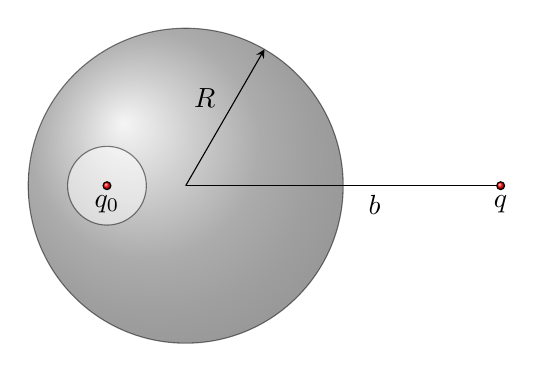
\begin{tikzpicture}
			\draw [ball color=gray, opacity=0.5] (0,0) circle (2);
			\draw [-stealth] (0,0) -- node[above left] {$R$} (60:2);
			\draw (0,0) -- node[below, pos =0.6] {$b$} (0:4);
			\draw [fill=white, opacity=0.5] (-1,0) circle (0.5);
			\draw [ball color=red] (-1,0) circle (0.05) node[below] {$q_0$};
			\draw [ball color=red] (0:4) circle (0.05) node[below] {$q$};
		\end{tikzpicture}
		\caption{До задачі~\ref{prb:charge_in_hole}}
		\label{charge_in_hole}
	\end{minipage}
	%---------------------------------------------------------
	\begin{minipage}[t]{0.45\linewidth}\centering
		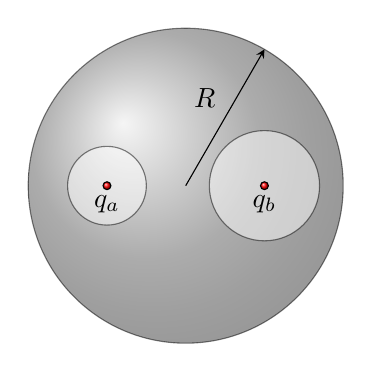
\begin{tikzpicture}
			\draw [ball color=gray, opacity=0.5] (0,0) circle (2);
			\draw [-stealth] (0,0) -- node[above left] {$R$} (60:2);
			\draw [fill=white, opacity=0.5] (-1,0) circle (0.5);
			\draw [ball color=red] (-1,0) circle (0.05) node[below] {$q_a$};
			\draw [fill=white, opacity=0.5] (1,0) circle (0.7);
			\draw [ball color=red] (1,0) circle (0.05) node[below] {$q_b$};
		\end{tikzpicture}
		\caption{До задачі~\ref{prb:charges_in_holes}}
		\label{charges_in_holes}
	\end{minipage}
	%---------------------------------------------------------
\end{figure}
%=========================================================
%=========================================================
\begin{problem}\label{prb:zobrazhnezazeml}
Точковий заряд $q$ знаходиться на відстані $b$ від центру металевої кулі радіусом $R$ ($ b > R$). Визначити силу взаємодії між зарядом і кулею. Розглянути випадки коли
\begin{enumerate*}[label=\alph*)]
	\item куля незаряджена і заземлена,
	\item куля незаряджена і незаземлена,
	\item куля несе заряд $Q$ і незаземлена.
\end{enumerate*}
Для всіх випадків проаналізувати отриманий вираз для сили при $b \gtrsim R$.
\begin{solution}
	\begin{enumerate*}[label=\alph*)]
		\item $F = \frac{q^2Rb}{(b^2-R^2)^2} $,
		\item $F = q^2R\left( \frac{b}{(b^2-R^2)^2} - \frac{1}{b^3}\right)$,
		\item $F = \frac{qQ}{b^2} - \frac{q^2R^3(2b^2 - R^2)}{b^3(b^2 - R^2)^2}$.
	\end{enumerate*}
\end{solution}
\end{problem}

%=========================================================
%\begin{problem}
%Частинка зарядом $q$ і масою $m$ знаходиться в положені рівноваги біля незаземленої металевої зарядженої кулі радіусом $R$ ($ b > R$). Заряд кулі дорівнює $Q$. Заряди частинки і кулі однойменні. Масу кулі вважати набагато більшою за масу частинки. Визначити період малих коливань частинки навколо положення рівноваги.
%\end{problem}



%=========================================================
\begin{problem}
Точковий заряд $q$ знаходиться на відстані $a$ від центру заземленої незарядженої металевої кулі радіусом $R$ ($ a < R$). Визначити силу взаємодії між зарядом і кулею. Як зміниться результат якщо куля буде незаземленою? Як зміниться результат якщо куля буде зарядженою?
\begin{solution}
	$F = -\frac{qRa}{(a^2 - R^2)^2}$. Якщо кулю буде незаземленою, результат не зміниться. Сила взаємодії не залежить від заряду кулі.
\end{solution}
\end{problem}


%=========================================================
\begin{problem} %КРС 3.8
Точковий заряд $q$ поміщений на відстані $\nfrac{R}{2}$ від центру тонкостінної металевої незаземленої сфери радіусом $R$, яка має заряд $-2q$. Визначити поверхневу густину заряду на внутрішній і зовнішній поверхнях сфери в точках, найбільш віддалених від цього заряду. Як зміниться результат, якщо сферу заземлити?
\begin{solution}
	$\sigma_{in} = \frac{q}{18\pi r^2}$, $\sigma_{out} = - \frac{q}{4\pi r^2}$. Після заземлення $\sigma_{in} = \frac{q}{18\pi r^2}$, $\sigma_{out} = 0$.
\end{solution}
\end{problem}

%=========================================================
\begin{problem}
Знайти розподіл зарядів на поверхні провідника, границя якого являє собою нескінченну площину з виступом у вигляді напівcфери радіусом $R$. Поверхнева густина заряду на великій відстані від виступу~$\sigma_0$.
\end{problem}

%=========================================================
\begin{problem}
Довга тонка дротина розташована паралельно осі довгого металевого циліндра радіусом $r$ на відстані $R > r$ від його осі. Лінійна густина заряду нитки $\lambda$, а циліндра $-\lambda$. Знайти силу взаємодії на одиницю довжини між провідниками.
\begin{solution}
	$F = \frac{2\lambda^2}{R\left( 1 - \nfrac{r^2}{R^2}\right) }$.
\end{solution}
\end{problem}

%=========================================================
\begin{problem}\label{prb:Ovch2.32}
На відстані $b= 10R$ від заземленої незарядженої металевої сфери радіусом $R$ розташований точковий електричний диполь з моментом $p$, причому вісь диполя перпендикулярна прямій, що сполучає центр сфери з серединою осі диполя (рис.~\ref{Ovch2.32}). Знайти силу взаємодії між диполем і сферою.
\begin{solution}
	$F = \frac{3p^2R^3}{b^7}$, взаємодія~--- притягування.
\end{solution}
\end{problem}
%---------------------------------------------------------
\begin{figure}[h!]\centering
	\begin{tikzpicture}
		\draw [ball color=gray, opacity=0.5] (0,0) circle (1);
		\draw [-latex] (4,-0.5) -- (4,0.5) node [above] {$\vect{p}$};
		\draw [-latex'] (0,0) -- node [right] {$R$}(135:1);
		\draw [latex'-latex'] (0,0) -- node [below] {$b$}(4,0);
		\draw (0,-1) -- (0,-1.5) coordinate (G);
		\draw (G) +(-0.5,0) -- +(0.5,0)
		+(-0.3,-0.1) -- +(0.3,-0.1)
		+(-0.1,-0.2) -- +(0.1,-0.2);
	\end{tikzpicture}
	\caption{До задачі~\ref{prb:Ovch2.32}}
	\label{Ovch2.32}
\end{figure}
%---------------------------------------------------------

%=========================================================
\begin{problem}
Заземлена металева куля радіусом $R$ лежить на тонкому рівномірно зарядженому діелектричному диску такого ж радіуса. Знайти заряд кулі, якщо заряд диска дорівнює~$q$.
\begin{solution}
	Згідно методу зображень, металева куля створює заряд-зображення $dq'$ елемента поверхні диска, на якому міститься заряд $dq = \sigma dS$, де $\sigma = \frac{q}{\pi R^2}$. Величину заряду-зображення (заряд кулі) можна знайти як:
	\[
		q' = - \int\frac{R}{r}\sigma dS.
	\]

	Для інтегрування, зручно скористатись елементом тілесного кута, під яким видно елемент диска з центру сфери:
	\[
		d\Omega = \frac{dS\cos\theta}{r^2}.
	\]

	Отже
	\[
		q' = - 2\pi R^2\int\limits_{0}^{\nfrac{\pi}{4}} \frac{\sin\theta}{\cos^2\theta}d\theta = -2(\sqrt2 - 1)q.
	\]
\end{solution}
\end{problem}


%=========================================================
\begin{problem}
Система двох тонких концентричних півкілець з зарядами $Q$ і $q$, та радіусами $r_1$ і $r_2$, поміщені в середину заземленої металевої сфери радіусом $R$, так, що центри кілець і кулі співпадають. Знайти потенціал у центрі сфери, якщо площини кілець перпендикулярні.
\begin{solution}
	$\phi = \frac{Q}{r_1} + \frac{q}{r_2} + \frac{Q+q}{R}$.
\end{solution}
\end{problem}


\section{Граничні умови. Поле у речовині}

\begin{Theory}\small

  Рівняння Максвелла для електростатичного поля в речовині:
  \begin{align}
	  \divg\Dfield & = 4\pi\rho, \label{divD}\\
	  \rot\Efield  & = 0. \tag{\ref{rotE}}
  \end{align}
  де $\rho$~-- густина вільних електричних зарядів.

  Теорема Гауса для вектора $\Efield$ в речовині:
  \begin{equation}
	  \oiint\limits_{S} \Efield d\vect{S} = 4\pi\left( \iiint\limits_V \rho dV + \iiint\limits_V \rho' dV\right) ,
  \end{equation}
  де $\rho$~-- густина вільних електричних зарядів,  $\rho'$~-- густина зв'язаних електричних зарядів.

  Поляризованість (вектор поляризації) $\vect{P}$~--- величина, що дорівнює дипольному моменту одиниці об'єму речовини:
	\begin{equation}
		\vect{P} = \frac{\vect{p}}{V}
	\end{equation}

  Теорема Гауса для поляризованості $\vect{P}$ (зв'язаний заряд, що з'являється на поверхні $S$ протилежний за знаком до заряду, що виникає в об'ємі $V$):
  \begin{equation}
	  \oiint\limits_{S} \vect{P} d\vect{S} = -  \iiint\limits_V \rho' dV.
  \end{equation}

  Диференціальна форма:
  \begin{equation}
	  \divg\vect{P} = - \rho',
  \end{equation}
  де $\rho'$~-- об'ємна густина зв'язаних електричних зарядів.


  Поверхнева густина зв'язаних електричних зарядів на межі розділу двох діелектриків:
  \begin{equation}
	  \sigma' = P_{1n} - P_{2n},
  \end{equation}
  де $\vect{n}$~-- вектор нормалі до поверхні розділу двох середовищ, що напрямлений з середовища $1$ в середовище $2$.

  Означення вектора електричної  індукції:
  \begin{equation}
	  \Dfield = \Efield + 4\pi\vect{P}
  \end{equation}

  Теорема Гауса для вектора $\Dfield$:
  \begin{equation}
	  \oiint\limits_{S} \Dfield d\vect{S} =  \iiint\limits_V \rho dV.
  \end{equation}

  Зв'язок між вектором поляризації (поляризованістю) та електричним полем, \emph{яке зумовило поляризацію} (у випадку ізотропних діелектриків):

  \begin{equation}
	  \vect{P} = \chi\Efield,
  \end{equation}
  де $\chi$~-- поляризовність діелектрика.

  \begin{equation}
	  \epsilon = 1 + 4\pi\chi,
  \end{equation}
  діелектрична проникність діелектрика.


  Граничні умови для векторів $\Efield$ та $\Dfield$:
  \begin{align}
	  E_{1\tau}       & = E_{2\tau},  \label{E_boundary} \\
	  D_{2n} - D_{1n} & = 4\pi\sigma, \label{D_boundary}
  \end{align}
  де $\sigma$~-- поверхнева густина вільних електричних зарядів на границі розділу діелектриків.
\end{Theory}

\subsection*{Принципові питання електростатики діелектриків}

%=========================================================
\begin{problem}
	Отримайте граничні умови~\ref{E_boundary} та \ref{D_boundary}.
\end{problem}


%=========================================================
\begin{problem}
	Довгий циліндр виготовлений з діелектрика з замороженою поляризованістю $\vect{P} = \const$, що напрямлена вздовж його осі. Зобразити схематичну картину полів вектора $\vect{D}$ та вектора $\vect{E}$ в середині та зовні циліндра.
\end{problem}

%=========================================================
\begin{problem}
	Довгий циліндр довжиною $2l$  і радіусом $r$ ($l \gg r$) виготовлений з діелектрика з замороженою поляризованістю $\vect{P} = \const$, що напрямлена вздовж його осі. Оцінити
	\begin{enumerate*}[label=\alph*)]
		\item величину і напрямок поля на основах зовні циліндра,
		\item величину і напрямок поля в центрі циліндра,
		\item величину і напрямок поля на зовнішній поверхні циліндра на середині його довжини.
	\end{enumerate*}
	\begin{solution}
		\begin{enumerate*}[label=\alph*)]
			\item $\vect{E} = \pm 2\pi \vect{P}$,
			\item $\vect{E} = -2\pi \vect{P} \left(\frac{r}{l} \right)^2$,
			\item величину і напрямок поля на поверхні циліндра поблизу його центра приблизно дорівнює полю в його центрі.
		\end{enumerate*}
		$\vect{E}_A = 4\pi \vect{P}$, $\vect{P}$
	\end{solution}
\end{problem}


%=========================================================
\begin{problem}
	Короткий циліндр (диск) товщиною $d$ і радіусом $R$ виготовлений з діелектрика з замороженою поляризованістю $\vect{P} = \const$, що напрямлена вздовж його осі. Оцінити поле зовні та в середині поблизу центра його основи. Визначити вектор індукції в цих точках.
	\begin{solution}
		Поле зовні $\vect{E} = 2\pi\vect{P}\frac{d}{R}$, поле в середині $\vect{E} = -2\pi\vect{P}\left( 2 - \frac{d}{R}\right) $.
		Індукція зовні та в середині $\vect{D} = 2\pi\vect{P}\frac{d}{R}$.
	\end{solution}
\end{problem}


%=========================================================
\begin{problem}
	Показати, що на межі розділу зарядженого провідника, густина поверхневих зарядів на якому $\sigma$ і однорідного діелектрика з діелектричною проникністю $\epsilon$, що поляризується під дією електричного поля провідника, густина зв'язаних зарядів $\sigma'$ визначається формулою:
	\[
		\sigma' = - \sigma\frac{\epsilon - 1}{\epsilon}.
	\]
\end{problem}


%=========================================================
\begin{problem}\label{prb:surface_of_dielectric}
	Поблизу плоскої поверхні однорідного діелектрика з діелектричною проникністю $\epsilon$ напруженість електричного поля в вакуумі дорівнює $\Efield_0$ і складає кут $\theta$ з нормаллю до поверхні (\ref{surface_of_dielectric}). Вважаючи поле зовні та в середині діелектрика однорідним, знайти \begin{enumerate*}[label=\alph*)]
		\item потік вектора $\Efield$ через сферу радіуса $R$, центр якої лежить на поверхні діелектрика,
		\item циркуляцію  вектора $\Dfield$ вздовж контура $\Gamma$ довжиною $l$, площина якого перпендикулярна до поверхні діелектрика.
	\end{enumerate*}
	\begin{solution}
	\begin{enumerate*}[label=\alph*)]
		\item $\oint\limits_{S} \Efield d\vect{S} = \frac{\epsilon  -1}{\epsilon} \pi R^2 E_0 \cos\theta$,
		\item $\oint\limits_{\Gamma} \Dfield d\vect{r} = - \left( \epsilon -1\right)  l E_0 \sin\theta$.
	\end{enumerate*}
	\end{solution}
\end{problem}

%---------------------------------------------------------
\begin{figure}[h!]\centering
	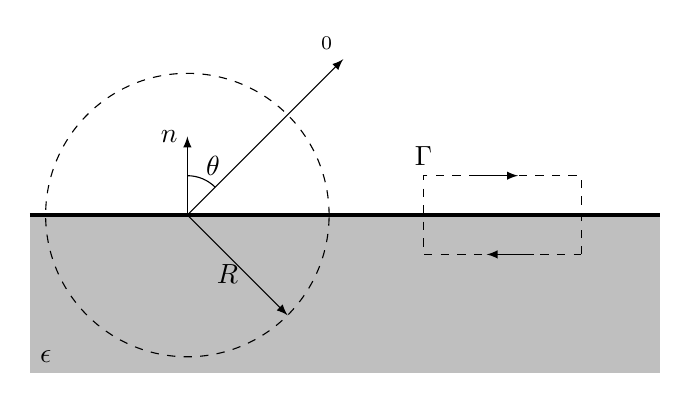
\begin{tikzpicture}[scale=2]
		\def\R{0.9}
		\fill[gray!50] (-2,-1) rectangle (2,0);
		\node at (-1.9,-0.9) {$\epsilon$};
		\draw[ultra thick] (-2,0) -- (2,0);
		\coordinate (P) at (-1,0);
		\coordinate (Q) at (1.5,0);
		\draw[dashed] (P) circle (\R);
		\draw[-latex] (P) -- node[pos=0.4, below] {$R$} +(-45:\R) ;
		\draw[-latex] (P) -- +(0,0.5) node[left] {$\vect{n}$};
		\draw[-latex] (P) -- +(45:{\R+0.5}) node[above left] {$\Efield_0$}  ;
		\draw (P) ++(45:0.25) arc (45:90:0.25) node[pos=0.1, above] {$\theta$};
		\draw[dashed] (Q) ++(0,-0.25) rectangle (0.5,0.25) node[above] {$\Gamma$};
		\draw[-latex] (Q)  ++(-0.7,0.25) -- +(0.3,0);
		\draw[-latex] (Q)  ++(-0.3,-0.25) -- +(-0.3,0);
	\end{tikzpicture}
	\caption{До задачі~\ref{prb:surface_of_dielectric}}
	\label{surface_of_dielectric}
\end{figure}
%---------------------------------------------------------


%=========================================================
\begin{problem}
	Знайти закон заломлення силових ліній на поверхні розділу двох діелектриків з проникностями $\epsilon_1$ та $\epsilon_2$. Зобразіть схематично картину заломлення однорідного поля на границі розділу для векторів $\vect{E}$ та $\vect{D}$.
	\begin{solution}
		$\epsilon_2 \tg\theta_1 = \epsilon_1 \tg\theta_2$, де $\theta_1$ та $\theta_2$~--- кути між нормаллю до поверхні та силовими лініями в діелектрику $1$ та $2$, відповідно.
	\end{solution}
\end{problem}


\subsection*{Знаходження напруженості електростатичного поля в діелектриках, які мають заморожену поляризованість}

%=========================================================
\begin{problem}\label{prb:Polarized_cylinder}
Знайти напруженість та індукцію електричного поля в центрі матеріалу, який має форму прямого круглого циліндра довжиною $l$ і радіусом $R$, поляризованість якого однорідна, напрямлена вздовж осі і дорівнює $ \vect{P} $.
\begin{solution}
	$\Efield = -4\pi \vect{P} \left( 1 - \frac{l}{\sqrt{4R^2 + l^2}}\right)$.
\end{solution}
\end{problem}

%=========================================================
\begin{problem}
Розв'язати задачу~\ref{prb:Polarized_cylinder}, у випадку, якщо поляризованість $ \vect{P} $ напрямлена перпендикулярно до осі циліндра.
\begin{solution}
	$\Efield = -2\pi \vect{P} \frac{l}{\sqrt{4R^2 + l^2}}$.
\end{solution}
\end{problem}

%=========================================================
\begin{problem}\label{prb:Field_of_Dielectric_Sphere}
Діелектрична куля радіусом $R$ поляризована однорідно з поляризованістю~$\vect{P}$. Знайти напруженість електричного поля всередині та зовні кулі.
\begin{solution}
	\[
	\Efield =
	\begin{cases}
	- \frac{4\pi}{3}\vect{P},                                                                                   & r \le R \\
	\frac{4\pi}{3}R^3\left( \frac{\vect{P}}{r^3} + \frac{3\left(\vect{P}\vect{r}\right)\vect{r} }{r^5}\right) , & r > R.
	\end{cases}
	\]
\end{solution}
\end{problem}

%=========================================================
\begin{problem}% Lim 2021
Нескінченно довгий діелектричний циліндр радіусом $R$ радіально поляризований таким чином, що поляризованість визначається законом $\vect{P}~=~a \vect{r}$, де $a$~-- позитивна константа. Знайти заряд, який припадає на одиницю довжини циліндра. Визначити напруженість та індукцію електричного поля в залежності від відстані до осі в середині та зовні циліндра.
\begin{solution}
	$\lambda = 0$,
	$\Dfield = 0$ у всьому просторі,
	$\Efield = %
		\begin{cases}
			- 4\pi  a  \vect{r}, & \quad r < R \\
			0,                              & \quad r > R
		\end{cases}
	$.
\end{solution}
\end{problem}

%=========================================================
\begin{problem}
	В середині плоского конденсатора, обкладки якого з'єднані між собою, вміщена діелектрична пластина товщиною $h$ з замороженою поляризованістю $\vect{P}$, що напрямлена перпендикулярно граням пластини і обкладкам конденсатора. Визначити модулі напруженості електричного поля та індукції зовні та в середині пластини. Відстань між пластинами конденсатора дорівнює $d$.
	\begin{solution}
		$E_1 = 4\pi P\frac{h}{d}$, $E_2  =4\pi P \left( 1 - \frac{h}{d}\right) $, $D_1 = D_2 = E_1$.
	\end{solution}
\end{problem}

\subsection*{Знаходження напруженості електростатичного поля  в діелектриках по заданому розподілу заряду}


%=========================================================
\begin{problem}
	Порожня металева куля, заряд якої $q$, а радіус $R$ плаває діелектричній рідині з проникністю $\epsilon$ так, що її центр знаходиться на рівні рідини. Знайти густину вільних зарядів на поверхні кулі.  Зобразіть схематично картину поля для векторів $\vect{E}$ та $\vect{D}$.
	\begin{solution}
		Заряди на поверхні кулі, яка знаходиться у вакуумі $\sigma_1 = \frac{q}{2\pi R (\epsilon + 1)}$, на поверхні, що занурена в діелектрик~--- $\sigma_2 = \epsilon \frac{q}{2\pi R (\epsilon + 1)}$.
		%=========================================================
		\begin{center}
			%---------------------------------------------------------
			\begin{minipage}[t]{0.45\linewidth}\centering
				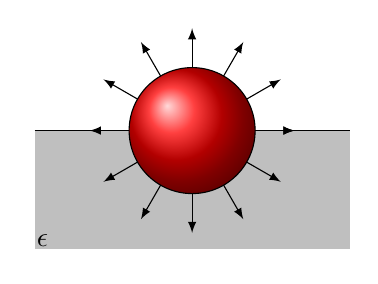
\begin{tikzpicture}
				\def\R{0.8}
				\fill[gray!50] (-2,-1.5) rectangle (2,0);
				\node at (-1.9,-1.4) {$\epsilon$};
				\draw[] (-2,0) -- (2,0);
				\coordinate (P) at (0,0);
				\foreach \i in {0,...,12} {\draw[-latex] (P) -- ({30*\i}:{\R+0.5});}
				\draw[ball color=red] (P) circle (\R);
				\end{tikzpicture}
				\captionof{figure}{Картина ліній вектора $\vect{E}$}
				\label{}
			\end{minipage}
			%---------------------------------------------------------
			\begin{minipage}[t]{0.45\linewidth}\centering
				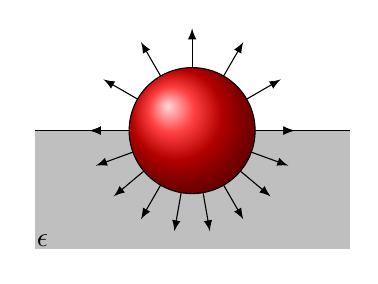
\begin{tikzpicture}
				\def\R{0.8}
				\fill[gray!50] (-2,-1.5) rectangle (2,0);
				\node at (-1.9,-1.4) {$\epsilon$};
				\draw[] (-2,0) -- (2,0);
				\coordinate (P) at (0,0);
				\foreach \i in {0,...,6} {\draw[-latex] (P) -- ({30*\i}:{\R+0.5});}
				\foreach \i in {9,...,18} {\draw[-latex] (P) -- ({20*\i}:{\R+0.5});}
				\draw[ball color=red] (P) circle (\R);
				\end{tikzpicture}
				\captionof{figure}{Картина ліній вектора $\vect{D}$}
			\end{minipage}
			%---------------------------------------------------------
		\end{center}
		%=========================================================
	\end{solution}
\end{problem}


%=========================================================
\begin{problem}
Точковий заряд $q$ розташований на плоскій границі розділу двох однорідних нескінченних діелектриків з проникностями $\epsilon_1$ і $\epsilon_2$. Знайти напруженість, індукцію і потенціал електричного поля у всьому просторі.
\begin{solution}
	$\phi = \frac{2}{\epsilon_1 + \epsilon_2} \frac{q}{r}$,
	$\Efield = \frac{2}{\epsilon_1 + \epsilon_2} \frac{q\vect{r}}{r^3}$,
	$\Dfield =
		\begin{cases}
			\frac{2\epsilon_1}{\epsilon_1 + \epsilon_2} \frac{q\vect{r}}{r^3}, & \text{в діелектрику 1} \\
			\frac{2\epsilon_2}{\epsilon_1 + \epsilon_2} \frac{q\vect{r}}{r^3}, & \text{в діелектрику 2}
		\end{cases}
	$
\end{solution}
\end{problem}


%=========================================================
\begin{problem}\label{prb:half_filled_condensator}
	Простір між обкладками плоского конденсатора заповнено повітрям, а напруженісь поля в зазорі дорівнює $E_0$. Потім половину зазору заповнюють діелектриком з проникністю $\epsilon$ так, що його поверхня в одному випадку  паралельна до обкладок, а в іншому перпендикулярна до обкладок.
	Знайти модулі векторів $\vect{E}$ та $\vect{D}$ для цих випадків, якщо
	\begin{enumerate*}[label=\alph*)]
		\item 	напруга між обкладками залишалась незмінною,
		\item 	заряд на обкладках залишався постійним.
	\end{enumerate*}
	\begin{solution}
		У випадку паралельного заповнення до обкладок:
		\begin{enumerate*}[label=\alph*)]
			\item за постійної напруги
			$E_1 = \frac{2\epsilon}{\epsilon + 1} E_0$, $E_2 = \frac{2}{\epsilon + 1} E_0$, $D_1 = D_2 = \frac{2\epsilon}{\epsilon + 1} E_0$;
			\item за постійного заряду
			$E_1 = E_0$, $E_2 = \frac{E_0}{\epsilon}$, $D_1 = D_2 = E_0$.
		\end{enumerate*}
		У випадку перпендикулярно заповнення до обкладок:
		\begin{enumerate*}[label=\alph*)]
			\item за постійної напруги
			$E_1 = E_2 = E_0$, $D_1 = E_0$, $D_2 = \epsilon D_1$;
			\item за постійного заряду
			$E_1 = E_2 = \frac{2}{\epsilon + 1} E_0$, $D_1 = \frac{2}{\epsilon + 1} E_0$, $D_2 = \epsilon D_1$.
		\end{enumerate*}
	\end{solution}
\end{problem}


\subsection*{Знаходження розподілу заряду по заданій напруженості електростатичного поля}

%=========================================================
\begin{problem}\label{FieldInDielectricSphere}
Однорідна куля радіусом $R$ з діелектричною проникністю $\epsilon$ вміщується в однорідне електричне поле напруженістю $\vect{E}_0$. Знайти дипольний момент кулі та напруженість електричного поля в усьому просторі, а також розподіл зв'язаних зарядів на кулі.
\begin{solution}
	$\vect{p} = \frac{\epsilon - 1}{\epsilon + 2}R^3\Efield_0$,
	$
		\Efield =
		\begin{cases}
			\frac{3}{\epsilon + 2} \Efield_0,                                                       & r \le R \\
			\Efield_0 + \frac{\vect{p}}{r^3} + \frac{3\left(\vect{p}\vect{r}\right)\vect{r} }{r^5}, & r > R
		\end{cases}
	$,
	$\sigma' = \frac{3}{4\pi} \frac{\epsilon - 1}{\epsilon + 2} \frac{\Efield_0\vect{r}}{r}$.
\end{solution}
\end{problem}

%=========================================================
\begin{problem}\label{FieldInDielectricHole}
В нескінченному діелектрику з проникністю $\epsilon$ створене однорідне поле напруженістю $\vect{E}_0$. В діелектрику вирізається сферична порожнина радіусом $R$. Знайти дипольний момент порожнини, поляризованість та напруженість електричного поля в усьому просторі після утворення порожнини, а також розподіл зв'язаних зарядів на поверхні порожнини.
\begin{solution}
	$\vect{p} = \frac{\frac{1}{\epsilon} - 1}{\frac{1}{\epsilon} + 2}R^3\Efield_0$,
	$\vect{P} = \frac{3}{4\pi} \frac{\frac{1}{\epsilon} - 1}{\frac{1}{\epsilon} + 2} \vect{E}_0$,
	$
		\Efield =
		\begin{cases}
			\frac{3}{\frac{1}{\epsilon} + 2} \Efield_0,                                             & r \le R \\
			\Efield_0 + \frac{\vect{p}}{r^3} + \frac{3\left(\vect{p}\vect{r}\right)\vect{r} }{r^5}, & r > R
		\end{cases}
	$.
\end{solution}
\end{problem}

%=========================================================
\begin{problem}[Узагальнений випадок задач \ref{FieldInDielectricSphere} та \ref{FieldInDielectricHole}]\label{sphere:Dielectric_in_Dielectric}%Черкасский
Однорідна куля радіусом $R$ з діелектричною проникністю $\epsilon_i$ занурена в однорідний необмежений діелектрик з діелектричною проникністю $\epsilon_e$. На великій відстані від кулі в діелектрику є однорідне електричне поле $\Efield_0$. Знайти дипольний момент кулі, потенціал і напруженість електричного поля в усьому просторі, а також розподіл зв'язаних зарядів на поверхні кулі.
\begin{solution}
	$\vect{p} = \frac{\epsilon_i - \epsilon_e}{\epsilon_i + 2\epsilon_e}R^3\Efield_0$,
	$
		\phi =
		\begin{cases}
			-\frac{3\epsilon_e}{\epsilon_e + 2\epsilon_e}\left( \Efield_0\cdot \vect{r}\right), & r \le R \\
			-\left( \Efield_0\cdot \vect{r}\right) + \frac{\vect{p} \vect{r}}{r^3},             & r > R
		\end{cases}
	$,\\
	$
		\Efield =
		\begin{cases}
			\frac{3\epsilon_e}{\epsilon_i + 2\epsilon_e} \Efield_0,                                 & r \le R \\
			\Efield_0 + \frac{\vect{p}}{r^3} + \frac{3\left(\vect{p}\vect{r}\right)\vect{r} }{r^5}, & r > R
		\end{cases}
	$,
	$\sigma' = \frac{3}{4\pi} \frac{\epsilon_i - \epsilon_e}{\epsilon_i + 2\epsilon_e} \frac{\Efield_0\vect{r}}{r}$.
\end{solution}
\end{problem}

\subsection*{Визначення густини поляризаційних зарядів в діелектрику та вектора поляризації}

%=========================================================
\begin{problem}
Визначити густину зв'язаних зарядів на поверхнях слюдяної пластинки ($\epsilon = 4.4$) товщиною $0.2$~мм, що є ізолятором у плоскому конденсаторі, різниця потенціалів на пластинах якого  дорівнює $400$~В.
\begin{solution}
	$\sigma' = 1.06\cdot10^{-8}$~К/см$^2$.
\end{solution}
\end{problem}

%=========================================================
\begin{problem} %Киселев
Металева сфера радіусом $R$, що несе заряд $q$, розташована в нескінченному однорідному діелектричному середовищі з проникністю $\epsilon$. Визначити поляризованість в довільній точці середовища, а також густини поверхневих і об'ємних зв'язаних зарядів в діелектрику.
\begin{solution}
	$\vect{P}(r) = \frac{1}{4\pi}\frac{\epsilon -1 }{\epsilon}\frac{q\vect{r}}{r^3}$,
	$\rho'=0$,
	$\sigma'=  - \frac{1}{4\pi}\frac{\epsilon -1 }{\epsilon}\frac{q}{R^2}$
\end{solution}
\end{problem}


%=========================================================
\begin{problem}
	Метал довільної форми, що має заряд $q$, оточений шаром однорідного діелектрика з проникністю $\epsilon$. Знайти сумарні поверхневі зв'язані заряди на внутрішній і зовнішній поверхнях діелектрика.
	\begin{solution}
		$q'_\text{внутр} = -q\frac{\epsilon - 1}{\epsilon}$, 	$q'_\text{зовн} = q\frac{\epsilon - 1}{\epsilon}$.
	\end{solution}
\end{problem}


%=========================================================
\begin{problem}
	В деякій точці в середині однорідного діелектрика з проникністю $\epsilon$ густина сторонніх зарядів $\rho$. Знайти в цій точці густину зв'язанних зарядів.
	\begin{solution}
		$\rho' = -\rho \frac{\epsilon - 1}{\epsilon}$.
	\end{solution}
\end{problem}


%=========================================================
\begin{problem}%Киселев
Точковий заряд $q$ знаходиться в центрі кулі радіусом $R$ з діелектрика з проникністю $\epsilon_1$. Куля оточена безмежним діелектриком з проникністю $\epsilon_2$. Знайти поверхневу густину зв'язаних зарядів на межі розділу цих діелектриків.
\begin{solution}
	$\sigma' = \frac{q}{4\pi R^2}\left( \frac{1}{\epsilon_2} - \frac{1}{\epsilon_1} \right) $
\end{solution}
\end{problem}

\subsection*{Метод електричних зображень для діелектриків}
%\begin{Theory}
%	Точковий заряд, який знаходиться на деякій відстані від поверхні розділу діелектриків, буде притягуватись до цієї поверхні, оскільки на ній індукуються зв'язані заряди протилежного знака. Розподіл заряду по поверхні ефективно можна моделювати ефективним зарядом-зображенням, який дорівнює величині~\cite[\S 24]{Siv3}:
%	\[
%		q' = - \frac{\epsilon_2 - \epsilon_1}{\epsilon_2 + \epsilon_1} q
%	\]
%	\begin{center}
%		\begin{tikzpicture};
%			\fill[gray!50] (0,-1) rectangle (4,0);
%			\fill[gray!10] (0,1) rectangle (4,0);
%			\draw[thick, gray] (0,0) -- (4,0);
%			\draw[-latex] (3,0) -- +(0,0.5) node[above] {$\vect{n}$};
%			\fill (2,-0.5) circle (0.05) node[right] {$q$};
%			\fill (2,+0.5) circle (0.05) node[right] {$q'$};
%			\node at (0.5,-0.5) {$\epsilon_1$};
%			\node at (0.5,0.5) {$\epsilon_2$};
%		\end{tikzpicture}
%	\end{center}
%\end{Theory}

%=========================================================
\begin{problem}
    Точковий заряд $q$ знаходиться в середовищі з діелектричною проникністю $\epsilon_1$ на відстані $d$ від границі розділу діелектриків. Діелектрична проникність другого діелектрика дорівнює $\epsilon_2$. Чому дорівнює сила, що діє на заряд? Від чого залежить напрямок цієї сили?
\begin{solution}
	$F = \frac{\epsilon_2 - \epsilon_1}{(\epsilon_2 + \epsilon_1)\epsilon_1} \frac{q}{4d^2}$.
\end{solution}
\end{problem}

%=========================================================
\begin{problem}%Журнал квант 2018, №5, стор. 9
    Два точкових заряди $q_1$ та $q_2$ знаходиться на однакових відстанях $d$ від границі розділу двох діелектриків з проникностями $\epsilon_1$ та $\epsilon_2$, відповідно. Знайдіть сили, що діють на кожен з зарядів. Проаналізуйте знак сил, що діють на заряди.
\begin{solution}
	$F_1 = \frac{\epsilon_1 - \epsilon_2}{(\epsilon_1 + \epsilon_2)\epsilon_1} \frac{q_1^2}{4d^2} + \frac{2}{\epsilon_1 + \epsilon_2} \frac{q_1q_2}{4d^2}$,
	$F_2 = \frac{\epsilon_2 - \epsilon_1}{(\epsilon_1 + \epsilon_2)\epsilon_2} \frac{q_2^2}{4d^2} + \frac{2}{\epsilon_1 + \epsilon_2} \frac{q_1q_2}{4d^2}$.
\end{solution}
\end{problem}

%=========================================================
%\begin{problem}\label{prb:dipole_under_dielectric}
%На відстані $d$ від півпростору, заповненого однорідним діелектриком з проникністю $\epsilon$, закріплений центр точкового диполя з дипольним моментом $\vect{p}$. Визначте силу взаємодії між диполем та діелектриком у випадку, якщо
%\begin{enumerate*}[label=\alph*)]
%	\item $\vect{p}$ перпендикулярний до поверхні діелектрика;
%	\item $\vect{p}$ паралельний до поверхні діелектрика.
%\end{enumerate*}
%\end{problem}

%=========================================================
\begin{problem}
Однорідний ізотропний діелектрик з проникністю $\epsilon$ заповнює весь нижній півпростір. У вакуумі на відстані $d$ від його поверхні знаходиться точковий заряд $q$. Визначити поверхневу густину поляризаційних (зв'язаних) зарядів в довільній точці на межі розділу, а також повний зв'язаний заряд на поверхні діелектрика. Який результат вийде, при $\epsilon\to\infty$, який це має фізичний зміст?
\begin{solution}
	$\sigma' = - \frac{\epsilon - 1}{\epsilon + 1} \frac{qd}{(x^2  +h^2)^{3/2}}$, де $x$~-- координата вздовж межі розділу, $q' = - \frac{\epsilon - 1}{\epsilon + 1}q$.
\end{solution}
\end{problem}

\section{Електрична ємність. Ємність взаємна, ємності коефіцієнти}

\begin{Theory}\small
	Означення електричної ємності:
	\begin{equation}\label{capacity}
		C = \frac{q}{\phi_1 - \phi_2}.
	\end{equation}

	Електрична ємність металевої сфери радіусу $R$:
	\begin{equation}\label{sphere_capacity}
		C = R.
	\end{equation}

	Електрична ємність плоского конденсатора ($S$ --- площа пластин, $d$~--- відстань між пластинами):
	\begin{equation}\label{condensator_capacity}
	C = \frac{\epsilon S}{4\pi d}.
	\end{equation}

	У випадку системи провідників, потенціал кожного з них залежить не тільки від заряду провідника, а визначається напруженостями, що створюються іншими провідниками, тобто від зарядів інших провідників, причому за принципом суперпозиції він прямо пропорційний цим зарядам. Наприклад, потенціал $i$-го провідника визначається як:
	\begin{equation}
		\phi_i = \sum\limits_{j=1}^{N}V_{ij} q_j,
	\end{equation}
	де $V_{ij}$~--- називаються потенціальними коефіцієнтами і утворюють потенціальну матрицю $\mathbb{V}$. Ємнісні коефіцієнти визначаються формою, розмірами та взаємним розташуванням провідників. Матриця, обернена до потенціальної $\mathbb{C} = \mathbb{V}^{-1}$ називається ємнісною матрицею, а її елементи $C_{ij}$~--- ємнісними коефіцієнтами:
	\begin{equation}\label{}
		q_i = \sum\limits_{j=1}^{N}C_{ij} \phi_j.
	\end{equation}
	Для потенціальних (та ємнісних) коефіцієнтів виконується теорема взаємності, яка говорить про те, що потенціальна (ємнісна) матриця є симетричною:
	\begin{equation*}\label{}
		V_{ij} = V_{ji}, \quad C_{ij} = C_{ji}
	\end{equation*}
	При чому:
	\begin{equation}\label{}
			V_{ii} > V_{ji} > 0, \quad C_{ii} >0, C_{ij}<0.
	\end{equation}
\end{Theory}

%=========================================================
\begin{problem}
    Чому ємність окремого провідника залежить від присутності поблизу інших провідників та їхнього розташування?

\end{problem}

%=========================================================
\begin{problem}
    Як зміниться ємність відокремленого провідника при появі поблизу іншого провідника?
\end{problem}

%=========================================================
\begin{problem}
    Чому ємність конденсатора не залежить від наявності оточуючих тіл чи електричних полів?
\end{problem}

%=========================================================
\begin{problem}
    У плоский повітряний конденсатор паралельно до обкладок вставляють діелектричну пластину, тоншу за зазор між обкладками. Як це вплине на ємність конденсатора? Чи залежатиме вона від положення пластини відносно обкладок?
\end{problem}

%=========================================================
\begin{problem}
    У плоский повітряний конденсатор паралельно до обкладок вставляють пластину діелектрика з проникністю $\epsilon$ і товщиною в половину зазору між обкладками. Як і в скільки разів зміниться ємність конденсатора?

\end{problem}

%=========================================================
\begin{problem}% Сивухін 148
Конденсатор приєднано до джерела постійної напруги. Чи зміниться напруженість електричного поля в конденсаторі, якщо його заповнити діелектриком? Як зміниться при цьому поверхнева густина вільних зарядів на обкладках конденсатора? Чому дорівнюватиме густина зв'язаних зарядів на поверхні діелектрика?
%\begin{solution}
%	Напруженість не зміниться.
%\end{solution}
\end{problem}

%=========================================================
\begin{problem}% Сивухін 112
Як зміниться напруженість поля між обкладками плоского конденсатора, якщо на одній з його обкладок заряд буде збільшено вдвічі?
\begin{solution}
	Збільшиться в $1.5$~рази.
\end{solution}
\end{problem}


%=========================================================
\begin{problem}\label{prb:shifted_plates}
Два однакові металеві диски діаметром $12$~см розташовані паралельно один до одного на відстані $0.2$~см. Диски зсунуті один відносно одного так, що центр одного з них  перебуває проти краю іншого (рис. \ref{shifted_plates}). Визначити ємність такої системи.
\begin{solution}
	$C \approx 70$~см.
\end{solution}
\end{problem}
%---------------------------------------------------------
\begin{figure}[h!]\centering
	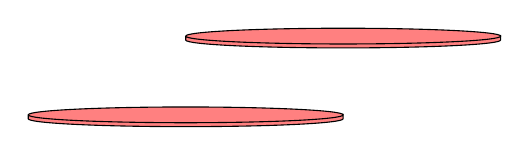
\begin{tikzpicture}
		\fill[red!50, draw=black] (-2,0.05) -- (-2,0) arc (180:360:2 and 0.1) -- +(0,0.05) arc (0:-180:2 and 0.1) arc (180:0:2 and 0.1) arc (0:-180:2 and 0.1);
		\fill[red!50, draw=black, yshift=-1cm,xshift=-2cm] (-2,0.05) -- (-2,0) arc (180:360:2 and 0.1) -- +(0,0.05) arc (0:-180:2 and 0.1) arc (180:0:2 and 0.1) arc (0:-180:2 and 0.1);
	\end{tikzpicture}
	\caption{До задачі~\ref{prb:shifted_plates}}
	\label{shifted_plates}
\end{figure}
%---------------------------------------------------------

%%=========================================================
%\begin{problem}% Lim 1041
%	Знайти ємність системи наведеній в  задачі~\ref{prb:3spheres_middle_ground}.
%\end{problem}
%
%%=========================================================
%\begin{problem}
%	Знайти ємність системи наведеній в задачі~\ref{prb:3spheres}.
%\end{problem}
%
%%=========================================================
%\begin{problem}% Lim 1041
%	Знайти ємність системи наведеній в задачі~\ref{prb:3spheres_and_ground}.
%\begin{solution}
%	$C = \frac{R_1R_3}{R_3 - R_1}$.
%\end{solution}
%\end{problem}

%=========================================================
\begin{problem}
    Дві концентричні металеві сфери мають радіуси $R_1$ та $R_2$ ($ R_2  > R_1 $). Внутрішню сферу заземлюють. Знайдіть ємність зовнішньої сфери.
\begin{solution}
	$C = \frac{R_2^2}{R_2 - R_1}$.
\end{solution}
\end{problem}

%=========================================================
\begin{problem}
Визначити наближено взаємну ємність системи, яка складається з двох  металевих куль радіусами $R_1$ та $R_2$, що знаходяться на дуже великій в порівнянні з їх радіусами відстані одна від одної. Система занурена в однорідний діелектрик проникністю $\epsilon$.
\begin{solution}
	$C \approx \frac{\epsilon R_1R_2}{R_1 + R_2}$.
\end{solution}
\end{problem}

%=========================================================
\begin{problem} % Батигін 132
Простір між обкладинками сферичного конденсатора частково заповнено діелектриком, який розташований в середині тілесного кута $\Omega$ з вершиною в центрі обкладок. Радіуси обкладок $R_1$  та $R_2$, проникність
діелектрика $\epsilon$. Знайти ємність конденсатора.
\begin{solution}
	$C =\frac{R_1R_2}{R_2 - R_1} \left( 1 + \frac{\epsilon - 1}{4\pi}\Omega\right) $.
\end{solution}
\end{problem}

%=========================================================
\begin{problem}% Батигін 134
Сферичний конденсатор з радіусами обкладок $R_1$ та $R_2$ заповнений
діелектриком, проникність якого залежить від відстані до центра $r$ за законом $\epsilon = aR_1^2/r$, де $a$~-- деяка позитивна константа. Знайти ємність такого конденсатора.
\begin{solution}
	$C = \frac{aR_1^2}{R_2 - R_1}$.
\end{solution}
\end{problem}

%=========================================================
\begin{problem}% Батигін 133
В середині сферичного конденсатора з радіусами обкладок $R_1$ та $R_2$ діелектрична проникність змінюється за законом:
\begin{equation*}
	\epsilon(r) = %
	\begin{cases}
		\epsilon_1, & \quad R_1 \le r < R, \\
		\epsilon_2, & \quad R \le r < R_2, \\
	\end{cases}
\end{equation*}
де $R$~-- деяка відстань $R_1 < R < R_2$.

Знайти ємність конденсатора, розподіл зв'язаних зарядів та повний заряд в діелектрику.
\begin{solution}
	$C = \left[ \frac{1}{\epsilon_1}\left( \frac{1}{R_1} - \frac{1}{R}\right) + \frac{1}{\epsilon_2}\left( \frac{1}{R} - \frac{1}{R_2}\right) \right]^{-1} $, зв'язані заряди знаходяться на границях розділу: $\sigma'_{R_1} = - \frac{q}{4\pi R_1^2}\frac{\epsilon_1 - 1}{\epsilon_1}$, $\sigma'_{R_2} =  \frac{q}{4\pi R_2^2}\frac{\epsilon_2 - 1}{\epsilon_2}$, $\sigma'_{R} = \frac{q}{4\pi R^2}\frac{\epsilon_1 - \epsilon_2}{\epsilon_1\epsilon_2}$.
\end{solution}
\end{problem}

%=========================================================
\begin{problem}% Батигін 135
Плоский конденсатор заповнений діелектриком, проникність якого змінюється за законом $\epsilon = a\frac{z + d}{d}$, де $a$, деяка позитивна константа, $d$~-- відстань між обкладками, вісь $z$~-- напрямлена перпендикулярно обкладкам, площа яких $S$. Нехтуючи крайовими ефектами, знайти ємність конденсатора та розподіл в ньому зв'язаних зарядів, якщо різниця потенціалів між обкладинками~$V$.
\begin{solution}
	$C = \frac{aS}{4\pi d\ln2}$, заряд обкладки конденсатора $\sigma = \frac{aV}{4\pi d\ln2}$, $\sigma'_{z=0} = -\sigma \left( 1 - \frac{1}{a} \right) $, $\sigma'_{z=d} = -\sigma \left( 1 - \frac{1}{2a} \right) $, $\rho' = -\frac{\sigma d}{a(z + d)^2}$.
\end{solution}
\end{problem}

%=========================================================
\begin{problem}
Визначити взаємну ємність системи, яка складається із металевої кулі радіусом $R$ і нескінченної металевої площини, яка  розташована на відстані $l$ від кулі. Вважати $l \gg R$.
\begin{solution}
	$C \approx R$.
\end{solution}
\end{problem}

%=========================================================
\begin{problem}
    Визначити ємнісні коефіцієнти для двох металевих куль з радіусами $R_1$ і $R_2$. Центри куль знаходяться на відстані $l \gg R_1,R_2$ один від одного.
\begin{solution}
	$C_{11} = \frac{R_1 l^2}{l^2 - R_1R_2}$, $C_{22}  = -\frac{lR_1R_2}{l^2 - R_1R_2}$, $C_{22} = \frac{R_2 l^2}{l^2 - R_1R_2}$.
\end{solution}
\end{problem}

%=========================================================
\begin{problem}\label{prb:4plates}%Mironova G.A., Brandt N.N., Saleckij A.M. E'lektrostatika v voprosax i zadachax (2izd., Lan', 2010)(ISBN 9785811410880)(ru)(288s)_PG_.pdf
    Визначте ємнісні коефіцієнти для чотирьох паралельних металевих пластин площею $S$, розташованих і з'єднаних так,
як показно на рис.~\ref{4plates}, за умови $d_1, d_2 \ll \sqrt{S}$.
\begin{solution}
	$C_{11} = \frac{S}{4\pi d_1}$, $C_{12} = -\frac{S}{4\pi d_1}$, $C_{22} = \frac{S}{4\pi}\left( \frac{1}{d_1} + \frac{1}{d_2} \right) $, $C_{13} = 0$, $C_{23} = -\frac{S}{4\pi d_2}$, $C_{33} = \frac{S}{4\pi d_2}$.
\end{solution}
\end{problem}
%---------------------------------------------------------
\begin{figure}[h!]\centering
    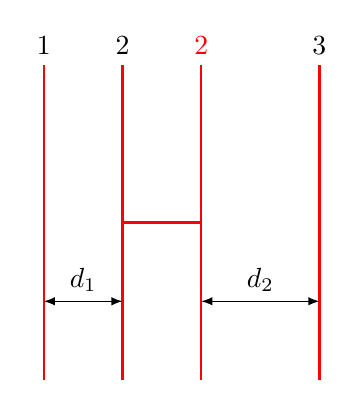
\begin{tikzpicture}
        \draw[thick, red] (-1,-2) -- (-1,2) node[above, text=black] {$1$};
		\draw[thick, red,] (0,-2) -- (0,2) node[above, text=black] {$2$};
		\draw[latex-latex] (-1,-1) -- node[above] {$d_1$} (0,-1);

        \draw[thick, red] (1,-2) -- (1,2) node[above] {$2$};
		\draw[thick, red,] (2.5,-2) -- (2.5,2) node[above, text=black] {$3$};
		\draw[latex-latex] (1,-1) -- node[above] {$d_2$} (2.5,-1);

		\draw[thick, red,] (0,0) -- (1,0);

    \end{tikzpicture}
\caption{До задачі~\ref{prb:4plates}}
\label{4plates}
\end{figure}
%---------------------------------------------------------



%=========================================================
\begin{problem}
Два довгих дроти радіусом $R$ кожен, розташовані паралельно один одному. Відстань між їх осями дорівнює $l$ ($l \gg R$). Знайти взаємну ємність одиниці довжини ділянки дротів.
\begin{solution}
	$C = \frac{1}{4\ln\frac{l - R}{R}}$.
\end{solution}
\end{problem}

%=========================================================
\begin{problem}% Купцов 2.25
Відімкнена від джерела дводротова лінія електропередачі знаходиться в однорідному полі грозової хмари з напруженістю $E_0 = 2$~кВ/м, яке напрямлене перпендикулярно поверхні землі. Один з дротів заземлений, інший~-- ізольований. Висота дротів над поверхнею $h = 5$~м, відстань між ними $d = 1$~м, а їх радіуси $R = 1$~см. Знайдіть потенціал ізольованого дроту.
\begin{solution}
	$\phi = E_0 h \left( 1 - \frac{\ln\frac{\sqrt{2h^2 + d^2}}{d}}{\ln\frac{2h}{R}}. \right) = 6.6$~кВ.
\end{solution}
\end{problem}

%=========================================================
\begin{problem}% Купцов 2.37
Два довгих дроти радіусом $R$ кожен, розташовані паралельно один одному на висоті $h$ над поверхнею Землі ($h \gg R$). Відстань між їх осями дорівнює $l$. Знайти взаємну ємність одиниці довжини ділянки дротів.
\begin{solution}
	$C = \frac{1}{4\ln\frac{2hl}{R\sqrt{d^2 + 2h^2}}}$.
\end{solution}
\end{problem}

%=========================================================
\begin{problem}
В середину порожнього тонкостінного і заземленого металевого циліндра радіусом $R$ вміщені два довгих паралельних дроти. Середина відстані між дротами співпадає з віссю циліндра. Радіус дротів $r$, відстань між ними $l$. Знайти взаємну ємність одиниці довжини лінії.
\begin{solution}
	$C = \frac14\ln^{-1}%
		\frac{%
			\left( \frac{2R^2}{l} - \frac{l}{2} + r \right)(l - r)
		}%
		{\left( \frac{2R^2}{l} + \frac{l}{2} - r \right)r }$.
\end{solution}
\end{problem}

\subsection*{Ємність систем конденсаторів}

%=========================================================
\begin{problem}
    Є кілька конденсаторів різної ємності. Як і що треба зробити, щоб отримати ємність:
	\begin{enumerate*}[label=\alph*)]
		\item меншу за найменшу з наявних;
		\item найменшу з усіх можливих;
		\item більшу за найбільшу з наявних;
		\item найбільшу з усіх можливих.
	\end{enumerate*}
\end{problem}

%=========================================================
\begin{problem}
    Скільки та якої величини різних ємностей можна ввімкнути між двома точками кола, маючи три конденсатори однакової ємності $C$?
\end{problem}

%=========================================================
\begin{problem}
    Конденсатор, ємністю $C_1 = 1$~мкФ витримує напругу не більше $V_1 = 6$~кВ, а конденсатор, ємністю $C_2 = 2$~мкФ~--- не більше $V_2 = 4$~кВ. Яку напругу може витримати система двох таких конденсаторів, з'єднаних послідовно?
\begin{solution}
	$9$~кВ.
\end{solution}
\end{problem}

%=========================================================
\begin{problem}\label{prb:section_of_circuin_with_condensators}
    Ділянка кола $AB$ (рис.~\ref{section_of_circuin_with_condensators}) містить джерело ЕРС $\EMF$ та два конденсатора ємностями $C_1$ та $C_2$. Різниця потенціалів на ділянці $\phi_A - \phi_B$. Знайдіть напругу на конденсаторах.
\begin{solution}
	$U_1 = \frac{\phi_A - \phi_B + \EMF}{C_1 + C_2} C_2$,
	$U_2 = \frac{\phi_A - \phi_B + \EMF}{C_1 + C_2} C_1$.
\end{solution}
\end{problem}

%=========================================================
\begin{problem}\label{prb:condensator_circuit}
    Знайдіть напругу на кожному з конденсаторів (рис.~\ref{condensator_circuit}).
\begin{solution}
	$V_1 = \frac{(\EMF_2 - \EMF_1) C_2}{C_1 + C_2}$, $V_1 = \frac{(\EMF_2 - \EMF_1) C_1}{C_1 + C_2}$.
\end{solution}
\end{problem}
%=========================================================
\begin{figure}[h!]\centering
%---------------------------------------------------------
\begin{minipage}[t]{0.45\linewidth}\centering
\begin{tikzpicture}
    \draw (3,0) node[ocontact] {} node[above] {$B$} to [capacitor={info={$C_2$}}] (2,0) to [battery={info={$\EMF$}}] (1,0) to [capacitor={info={$C_1$}}] (0,0) node[ocontact] {} node[above] {$A$};
	\node[white] at (0,-1) {};
\end{tikzpicture}
\caption{До задачі~\ref{prb:infty_capacitor_chain}}
\label{section_of_circuin_with_condensators}
\end{minipage}
%---------------------------------------------------------
\begin{minipage}[t]{0.45\linewidth}\centering
	\begin{tikzpicture}
		\draw (0,0) to [capacitor={info'={$C_1$}}] ++(2,0)
		to [battery={info'={$\EMF_2$}, rotate=180}] ++(0,-2)
		to [capacitor={info'={$C_2$}}] ++(-2,0)
		to [battery={info={$\EMF_1$}}] ++(0,2);
	\end{tikzpicture}
\caption{До задачі~\ref{prb:condensator_circuit}}
\label{condensator_circuit}
\end{minipage}
%---------------------------------------------------------
\end{figure}
%=========================================================
\begin{problem}\label{prb:Irodov2.125}
В схемі, яка наведена на рис.~\ref{Irodov2.125} знайти різницю потенціалів між точками $A$ та $B$, якщо ЕРС джерела дорівнює $\EMF$, а відношення ємностей $C_2/C_1 = \eta$.
\begin{solution}
	$V = \EMF/ (1 + 3\eta + \eta^2)$.
\end{solution}
\end{problem}

%=========================================================
\begin{problem}\label{prb:infty_capacitor_chain}
Знайти ємність нескінченного кола, яке утворене повторенням однієї і тієї ж ланки з двох однакових конденсаторів, кожен з яких має ємність $C$ (рис.~\ref{infty_capacitor_chain}).
\begin{solution}
	$C_\text{ланки} = C \left( \sqrt5 -1 \right)/2$.
\end{solution}
\end{problem}

%=========================================================
\begin{figure}[h!]\centering
%---------------------------------------------------------
\begin{minipage}[t]{0.45\linewidth}\centering
	\begin{tikzpicture}
		\draw (0,2) to [battery={info'={$\EMF$}}] (0,0);
		\draw (0,2) to [capacitor={info={$C_1$}}] ++(2,0) node [contact] (A) {} to [capacitor={info={$C_1$}}] ++(2,0) node [contact] (A1) {} -- ++(1,0) node [ocontact] {} node [right]{$A$};
		\draw (0,0) -- ++(2,0) node [contact] (B) {} -- ++(2,0) node [contact] (B1) {} -- ++(1,0) node [ocontact] {} node [right]{$B$};
		\draw (A) to [capacitor={info={$C_2$}}] (B) (A1) to [capacitor={info={$C_2$}}] (B1);
	\end{tikzpicture}
	\caption{До задачі~\ref{prb:Irodov2.125}}
	\label{Irodov2.125}
\end{minipage}
%---------------------------------------------------------
\begin{minipage}[t]{0.45\linewidth}\centering
	\begin{tikzpicture}
		\draw (0,0) node[ocontact] {} to [capacitor={info={$C$}}] (2,0) node[contact] (A1) {} to [capacitor={info={$C$}}] (4,0) node[contact] (A2) {}  to [capacitor={info={$C$}}] (6,0) node[contact] (A3) {};
		\draw (0,-2) node[ocontact] {} -- (2,-2) node[contact] (B1) {} -- (4,-2) node[contact] (B2) {} -- (6,-2) node[contact] (B3) {};
		\draw (A1) to [capacitor={info={$C$}}] (B1) (A2) to [capacitor={info={$C$}}] (B2) (A3) to [capacitor={info={$C$}}] (B3);
		\draw [dashed] (A3) -- (8,0)
		(B3) -- (8,-2);
		\node[left] at (0,0) {$A$};
		\node[left] at (0,-2) {$B$};
		\node[] at (8,-1) {$\infty$};
	\end{tikzpicture}
	\caption{До задачі~\ref{prb:infty_capacitor_chain}}
	\label{infty_capacitor_chain}
\end{minipage}
%---------------------------------------------------------
\end{figure}
%=========================================================


%=========================================================
\begin{problem}\label{prb:Irodov2.129}
Знайти різницю потенціалів $\phi_A - \phi_B$ між точками $A$
та $B$ системи, яка показана:
\begin{enumerate*}[label=\alph*)]
	\item на рис~\ref{Irodov2.129-1},
	\item на рис~\ref{Irodov2.129-2}.
\end{enumerate*}
\begin{solution}
	\begin{enumerate*}[label=\alph*)]
		\item $\phi_A - \phi_B = \EMF\frac{C_2C_3 - C_1C_4}{\left( C_1 + C_2 \right)\left( C_3 + C_4 \right)}$,
		\item $\phi_A - \phi_B = \frac{\EMF_2C_2 - \EMF_1C_1}{\left( C_1 + C_2 + C_3 \right)}$.
	\end{enumerate*}
\end{solution}
\end{problem}

%=========================================================
\begin{figure}[htbp!]\centering
	%---------------------------------------------------------
	\begin{minipage}[t]{0.45\linewidth}\centering
		\begin{tikzpicture}
			\draw (4,0) coordinate (B) to [battery={info={$\EMF$}}] (0,0) coordinate (A);
			\draw (A) -- ++(0,1) node [contact] (C) {} -- ++(0,1)
			to [capacitor={info={$C_1$}}] ++(2,0) node[ocontact] {} node[above] {$A$}
			to [capacitor={info={$C_2$}}] ++(2,0) -- ++(0,-1) node [contact] (D) {} -- (B)
			(C) to [capacitor={info'={$C_3$}}] ++(2,0) node[ocontact] {} node[below] {$B$}
			to [capacitor={info'={$C_4$}}] (D);
		\end{tikzpicture}
		\caption{До задачі~\ref{prb:Irodov2.129}}
		\label{Irodov2.129-1}
	\end{minipage}
	%---------------------------------------------------------
	\begin{minipage}[t]{0.45\linewidth}\centering
		\begin{tikzpicture}
			\draw (4,0) coordinate (B) to [battery={info={$\EMF_2$}}] (2,0) node[contact] (B1) {} node [below] {$B$}  to [battery={info={$\EMF_1$}}] (0,0) coordinate (A)
			(A) -- ++(0,2) to [capacitor={info={$C_1$}}] ++(2,0) node[contact] (A1) {} node [above] {$A$} to [capacitor={info={$C_2$}}] ++(2,0) -- (B)
			(A1) to [capacitor={info'={$C_3$}}] (B1)
			;

		\end{tikzpicture}
		\caption{До задачі~\ref{prb:Irodov2.129}}
		\label{Irodov2.129-2}
	\end{minipage}
	%---------------------------------------------------------
\end{figure}
%=========================================================

%=========================================================
\begin{problem}
    До джерела ЕРС $\EMF$ послідовно приєднали два повітряні конденсатори, кожен ємністю $C$. Потім один з конденсаторів заповнили діелектриком проникністю $3$. У скільки разів зменшилась напруженість електричного поля у цьому конденсаторі? Який заряд пройде через джерело?
\begin{solution}
	Напруженість зменшиться у $\frac{1 + \epsilon}{2}$ рази. Заряд, що пройде через джерело $\frac12 C\EMF \frac{\epsilon - 1}{\epsilon  +1}$.
\end{solution}
\end{problem}

%=========================================================
\begin{problem}
    Конденсатор ємністю $C_1$~мкФ, заряджений до напруги $V$, приєднали до кінців системи з двох послідовно з'єднаних незаряджених конденсаторів, ємності яких $C_2$ і $C_3$. Який заряд пройде при цьому по підвідних провідниках?
\begin{solution}
	$q = V \frac{C_1C_2C_3}{C_1C_2 + C_2C_3 + C_1C_3}$.
\end{solution}
\end{problem}

%=========================================================
\begin{problem}\label{prb:cond_scheme}
	 Які заряди пройдуть після замикання ключа у схемах поданих на
	\begin{enumerate*}[label=\alph*)]
		\item рис.~\ref{cond_scheme1} та
		\item рис.~\ref{cond_scheme2}
	\end{enumerate*}
	через напрямки, казані стрілками.
	На схемах ЕРС кожного з джерел $\EMF = 60$~В, ємності конденсаторів $C_1 = 2$~мкФ та $C_2 = 3$~мкФ.
\begin{solution}
	\begin{enumerate*}[label=\alph*)]
		\item $\Delta q_1 = \EMF C_2$, $\Delta q_2 = -\frac{C_1C_2}{C_1 + C_2}\EMF$,
		\item $\Delta q_1 = \frac{C_1 - C_2}{C_1 + C_2}\EMF С_1$, $\Delta q_2 = \EMF(C_1 - C_2)$.
	\end{enumerate*}
\end{solution}
\end{problem}

%=========================================================
\begin{figure}[h!]\centering
%---------------------------------------------------------
\begin{minipage}[t]{0.45\linewidth}\centering
	\begin{tikzpicture}
			\draw (4,0) coordinate (B) -- (2,0) node[contact] (B1) {} node [below] {$B$}  -- (0,0) coordinate (A)
			(A) to [battery={info'={$\EMF_1$}, rotate=180}]  ++(0,2) to [make contact] ++(2,0) node[contact] (A1) {} node [above] {$A$} to [capacitor={info={$C_1$}}] ++(2,0) to [battery={info={$\EMF_2$}}] (B)
			(A1) to [capacitor={info'={$C_2$}}] (B1)
			;
			\draw[-latex, red] (2.5,0) -- +(0.5,0) node[above, black] {$2$};
			\draw[-latex, red] (1.5,0) -- +(-0.5,0) node[above, black] {$1$};
	\end{tikzpicture}
\caption{До задачі~\ref{prb:cond_scheme}}
\label{cond_scheme1}
\end{minipage}
%---------------------------------------------------------
\begin{minipage}[t]{0.45\linewidth}\centering
	\begin{tikzpicture}
			\draw (4,0) coordinate (B) -- (2,0) node[contact] (B1) {} node [below] {$B$}  -- (0,0) coordinate (A)
			(A) to [battery={info'={$\EMF_1$}, rotate=180}]  ++(0,2) to [capacitor={info={$C_1$}}] ++(2,0) node[contact] (A1) {} node [above] {$A$} to [capacitor={info={$C_2$}}] ++(2,0) to [battery={info={$\EMF_2$}}] (B)
			(A1) to [make contact] +(0,-1) --  (B1)
			;
			\draw[-latex, red] (2,0.5) -- +(0,0.5) node[right, black] {$2$};
			\draw[-latex, red] (1.5,0) -- +(-0.5,0) node[above, black] {$1$};
	\end{tikzpicture}
\caption{До задачі~\ref{prb:cond_scheme}}
\label{cond_scheme2}
\end{minipage}
%---------------------------------------------------------
\end{figure}
%=========================================================

%=========================================================
\begin{problem}\label{prb:Zhurnal_Kvant_2000_1_6}%Журнл Квант, 2000, №1, задача 6, #55
    Батарею паралельно з'єднаних конденсаторів з ємностями $C_1 = 1$~мкФ і $C_2 = 2$~мкФ спочатку під'єднали до джерела з ЕРС, яка дорівнює $\EMF = 6$~В (ключ в положенні $1$ на рис.~\ref{Zhurnal_Kvant_2000_1_6}). Потім ключ переводять в положення $2$, поєднуючи батарею з конденсатором ємністю $C_3 = 3$~мкФ. Знайдіть заряд, який отримає конденсатор ємністю $C_3$.
\begin{solution}
	$q_3 = \EMF C_3 \frac{C_1 + C_2}{C_1 + C_2 + C_3} = 9$~мкФ.
\end{solution}
\end{problem}


%=========================================================
\begin{problem}\label{prb:Zhurnal_Kvant_2018_9_F2524}
    Незаряджений плоский конденсатор ємністю $C_1$ розташований в зовнішньому однорідному електричному полі $E_0$, перпендикулярному до площин його обкладок (див.~\ref{Zhurnal_Kvant_2018_9_F2524}). Відстань між обкладинками $d$. Конденсатор ємністю $C_2$, що несе на своїх пластинах заряди $\pm q_0$ (плюс на обкладанні ліворуч), підключається до першого конденсатору. Визначте заряди $q_1$ і $q_2$ на лівих пластинах конденсаторів після підключення. Впливом зовнішнього електричного поля в місці знаходження другого конденсатора знехтувати.
\begin{solution}
	$q_1 = C\left( \frac{q_0}{C_2} - E_0 d\right) $,
	$q_2 = C\left( \frac{q_0}{C_1} - E_0 d\right) $, де $C = \frac{C_1C_2}{C_1 + C_2}$.
\end{solution}
\end{problem}

%=========================================================
\begin{figure}[h!]\centering
%---------------------------------------------------------
\begin{minipage}[t]{0.45\linewidth}\centering
	\begin{tikzpicture}
		\draw (0,0) to[battery={info'={$\EMF$}, rotate=180}] ++(0,3) -- ++(1.5,0) node[contact] {} node[above] {$1$} coordinate (A); \draw ([xshift=1cm]A) node[contact] {} node[above] {$2$} -- ++(1.5,0) to[capacitor={info'={$C_3$}}] ++(0,-3) -- ++(-2,0) node[contact] {} coordinate (B) -- (0,0);
		\draw (B) -- ++(0,0.75) -- ++(-0.75,0)  to[capacitor={info={$C_1$}}] ++(0,1.5) -- ++(+0.75,0) -- ++(0,0.5) -- (A);
		\draw (B) -- ++(0,0.75) -- ++(+0.75,0)  to[capacitor={info={$C_2$}}] ++(0,1.5) -- ++(-0.75,0);
	\end{tikzpicture}
\caption{До задачі~\ref{prb:Zhurnal_Kvant_2000_1_6}}
\label{Zhurnal_Kvant_2000_1_6}
\end{minipage}
%---------------------------------------------------------
\begin{minipage}[t]{0.45\linewidth}\centering
	\begin{tikzpicture}
		\draw node[ocontact] {} (0,0) -- (0,1) to [capacitor={info={$C_1$}}]  (4,1) -- (4,0) node[ocontact] {};
		\foreach \i in {0.6,0.8,...,1.4}{
		\draw[-latex,red] (0,\i) -- (4,\i);
		}
		\node[right] at (4,1.4) {$E_0$};
		\draw[latex-] (0,-0.5) -- ++(0,-1) coordinate (A);
		\draw (A) to [capacitor={info={$C_2$}}]  ++(4,0) coordinate (B) ;
		\draw[-latex] (B) -- ++(0,1);
	\end{tikzpicture}
\caption{До задачі~\ref{prb:Zhurnal_Kvant_2018_9_F2524}}
\label{Zhurnal_Kvant_2018_9_F2524}
\end{minipage}
%---------------------------------------------------------
\end{figure}
%=========================================================



\section{Енергія електричного поля}

\begin{Theory}\small
Енергія системи заряджених частинок:
\begin{equation}
	W = \frac12\sum\limits_i q_i \phi_i,
\end{equation}
де $\phi_i$~--- потенціал, в якому перебуває частинка зарядом $q_i$.

Власна електростатична енергія зарядженого тіла:
\begin{equation}
	W = \frac12\iiint\limits_{V}\rho\phi dV + \frac12\iint\limits_{S}\sigma\phi dS,
\end{equation}
де $\rho$ та $\sigma$~-- об'ємна та поверхнева густини вільних електричних зарядів, відповідно.

Енергія жорсткого диполя в електричному полі:
\begin{equation}
	W = -\vect{p}\cdot\Efield.
\end{equation}

Енергія квазіпружного диполя в електричному полі:
\begin{equation}
	W = -\frac12 \left( \vect{p}\cdot\Efield \right) .
\end{equation}

Енергія зарядженого конденсатора:
\begin{equation}
	W = \frac{CV^2}{2} = \frac{q^2}{2C}.
\end{equation}

Густина енергії електричного поля:
\begin{equation}
	w = \frac{\Dfield\cdot\Efield}{8\pi}.
\end{equation}

Енергія електростатичного поля:
\begin{equation}
	W = \iiint\limits_V  \frac{\Dfield\cdot\Efield}{8\pi} dV
\end{equation}
\end{Theory}


\subsection*{Визначення енергії системи заряджених частинок та диполів}

%=========================================================
\begin{problem}\label{prb:qseq}
Обчислити енергію нескінченного лінійного ланцюжку точкових зарядів, величина яких дорівнює $q$, а знаки чергуються. Відстань між сусідніми різнойменними зарядами дорівнює $a$ (рис.~\ref{qseq}).
\begin{solution}
	$W = - \frac{2q^2}{a}$
\end{solution}
\end{problem}
%---------------------------------------------------------
\begin{figure}[h!]\centering
	\begin{tikzpicture}
		\coordinate(A) at (0,0);
		\node at ([xshift=-1cm]A) {$\ldots$};
		\node at ([xshift=11cm]A) {$\ldots$};
		\foreach \i in {0,1,2,3,4,5}  {
				\ifodd\i\def\sign{+}\def\col{red}\else\def\sign{-}\def\col{blue}\fi
				\fill[\col] (2*\i,0) circle (0.1) node[below, black] {$\sign q$};
			}
		\draw[] (4,0) -- (4,0.6);
		\draw[] (6,0) -- (6,0.6);
		\draw[latex-latex] (4,0.5) -- node[above] {$a$} (6,0.5);
	\end{tikzpicture}
	\caption{До задачі~\ref{prb:qseq}}
	\label{qseq}
\end{figure}
%---------------------------------------------------------

%=========================================================
\begin{problem}
    Знайти електростатичну енергію іонного кристалу\ce{NaCl}. Кристалічна гратка \ce{NaCl} кубічна з відстанню між сусідніми однозарядними йонами \ce{Na} та \ce{Cl} дорівнює $a = 2.81\,\AA$.
\begin{solution}
	$W = -1.747\frac{e^2}{a} = -8.94$~еВ.
\end{solution}
\end{problem}

%=========================================================
\begin{problem}\label{prb:twodip}
Два диполя з моментами $\vect{p_1}$ і $\vect{p_2}$, які лежать в одній площині на відстані $d$ один від одного, утворюють з прямою, яка з'єднує диполі, кути $\theta_1$ і $\theta_2$ відповідно (рис.~\ref{twodip}). Обчислити енергію взаємодії диполів. Знайти кути, при яких енергія буде
\begin{enumerate*}[label=\alph*)]
	\item максимальною,
	\item дорівнюватиме нулю та
	\item мінімальною.
\end{enumerate*}
\begin{solution}
	$W = -(\vect{p}_1\cdot \Efield_2) = -\frac{3(\vect{p}_1\cdot\vect{r})(\vect{p}_2\cdot\vect{r})}{r^5}  + \frac{(\vect{p}_1\cdot\vect{p}_2)}{r^3}= -\frac{p_1p_2}{d^3}\left[ 3\cos\theta_1\cos\theta_2 - \cos(\theta_1 - \theta_2)\right] $,
	\begin{enumerate*}[label=\alph*)]
		\item $\theta_1 = \theta_2 = \pi/2$,
		\item $\theta_1 =0$, $\theta_2 =\pi/2$,
		\item $\theta_1 = \theta_2 = 0$.
	\end{enumerate*}
\end{solution}
\end{problem}

%=========================================================
\begin{problem}\label{prb:dipole_in_field}
На відстані $d$ від півпростору, заповненого однорідним діелектриком з проникністю $\epsilon$, закріплений центр точкового диполя з дипольним моментом $\vect{p}$. Диполь може вільно обертатися, змінюючи напрямок. Паралельно межі півпростору прикладене однорідне зовнішнє електричне поле $\Efield$ (рис.~\ref{dipole_in_field}). Знайти встановлене рівноважне значення кута $\alpha$ між напрямком векторів $\Efield$ і $\vect{p}$.
\begin{solution}
	В діелектрику виникає зображення диполя, з моментом $\vect{p}' = -\vect{p}\frac{\epsilon - 1}{\epsilon + 1}$. Кут між полем $\Efield$ і диполем $\vect{p}'$ дорівнює $\pi - \alpha$.

	Сумарний момент сил, що діє на диполь
    \[
        \left[\vect{p}\times\Efield\right] + \left[\vect{p}\times\left( \frac{3(\vect{p}'\vect{r})\vect{r}}{r^5} - \frac{\vect{p}'}{r^3} \right) \right] = 0
    \]

	Звідки,  можливі наступні випадки $\alpha = 0$, та $\alpha = \pm\arccos\left( -\frac{E}{\frac{\epsilon - 1}{\epsilon + 1} \frac38\frac{p}{d^3}}\right) $.
\end{solution}
\end{problem}

%=========================================================
\begin{figure}[h!]\centering
	%---------------------------------------------------------
	\begin{minipage}[t]{0.45\linewidth}\centering
		\begin{tikzpicture}
			\draw [dash dot] (-1,0) -- (6,0);
			\draw[-latex, ultra thick, red] (0.5,0) -- (60:1.5) node[above, black] {$\vect{p_1}$};
			\draw (1,0) arc (0:60:0.7) node[pos=0.7, right] {$\theta_1$};
			\draw[-latex, ultra thick, red] (4.5,0) -- +(50:1) node[above, black] {$\vect{p_2}$};
			\draw (5,0) arc (0:39:0.7) node[pos=0.6, right] {$\theta_2$};
			\draw (0.5,0) -- (0.5,-0.4);
			\draw (4.5,0) -- (4.5,-0.4);
			\draw[latex-latex] (0.5,-0.3) -- node[below] {$d$} (4.5,-0.3);
		\end{tikzpicture}
		\caption{До задачі~\ref{prb:twodip}}
		\label{twodip}
	\end{minipage}
	%---------------------------------------------------------
	\begin{minipage}[t]{0.45\linewidth}\centering
		\begin{tikzpicture}%[scale=1.5]
			\draw[ultra thick] (-2,0) -- (2,0);
			\fill[gray!50] (-2,-1) rectangle (2,0);
			\node at (-1.5,-0.5) {$\epsilon$};
            \coordinate (A) at (0,2);
			\draw[-latex', thick, red] (A) +(-90+45:1) -- (A) -- ++(90+45:1) node[black, above] {$\vect{p}$};
			\draw[thin, dash dot] (A) -- ([xshift=0.7cm]A) coordinate[pos=0.8] (B);
			\draw[thin] (B) arc (0:90+45:0.55) node[pos=0.5, above] {$\alpha$};
			\draw[thin, dash dot] (A) -- node [right] {$d$} (A|-0,0);
			\draw[-latex] ([xshift=-2cm]A) -- node[below] {$\Efield$} ([xshift=-0.25cm]A) ;
		\end{tikzpicture}
		\caption{До задачі~\ref{prb:dipole_in_field}}
		\label{dipole_in_field}
	\end{minipage}
	%---------------------------------------------------------
\end{figure}
%=========================================================

\subsection*{Визначення електростатичної енергії заряджених тіл та конденсаторів}

%=========================================================
\begin{problem}
    Покажіть, що енергія провідника довільної форми, потенціал якого $\phi$, що несе заряд $Q$ дорівнює:
	\begin{equation*}
		W = \frac{1}{2}Q\phi
	\end{equation*}
\end{problem}

%=========================================================
\begin{problem}
    Нехай система складається з $N$ провідників, заряди яких $Q_i$ а потенціали на них $\phi_i$. Чому дорівнює енергія системи цих провідників?
\end{problem}

%=========================================================
\begin{problem}
    Система складаються із двох провідників довільної форми, які розташовані на відстані, що перевищує суму їх характерних лінійних розмірів. Один з провідників є заряджений, інший незаряджений. Тіла починають квазістатично (нескінченно повільно) зближувати, як при цьому змінюватиметься
	\begin{enumerate*}[label=\alph*)]
		\item  потенціал зарядженого провідника,
		\item  потенціал незарядженого провідника,
		\item різниця потенціалів між провідниками?
	\end{enumerate*}
\end{problem}


%=========================================================
\begin{problem}
Знайдіть енергію системи, яка розглянута в задачі~\ref{connecting_spheres} до і після з'єднання дротом. Поясніть результат з точки зору закону збереження енергії.
\end{problem}

%=========================================================
\begin{problem}% Іродов 2.141
Система складається з двох концентричних тонких металевих оболонок з радіусами $R_1$ і $R_2$ і відповідними зарядами $q_1$ і $q_2$. Знайти власну енергію кожної оболонки, енергію взаємодії оболонок і повну електричну енергію системи.
\begin{solution}
	$W_1 = \frac{q_1^2}{2R_1}$, $W_2 = \frac{q_1^2}{2R_1}$, $W_{12} = \frac{q_1q_2}{R_2}$, $W = W_1 + W_2 + W_{12}$.
\end{solution}
\end{problem}

%=========================================================
\begin{problem}
Металева сфера радіусом $R$, що має заряд $q$, занурена на половину в нескінченний ізотропний діелектрик з проникністю $\epsilon$.
Знайти енергію електростатичного поля.
\begin{solution}
	$W = \frac{q^2}{(\epsilon + 1)R}$.
\end{solution}
\end{problem}

%=========================================================
\begin{problem}
Центр незарядженої металевої сфери радіусом $R$ розташований на плоскій границі двох ізотропних діелектриків з проникностями $\epsilon_1$ і $\epsilon_2$. В середині сфери на відстані від її центру знаходиться точковий заряд $q$. Визначити енергію поля поза сферою.
\begin{solution}
	$W = \frac{q^2}{(\epsilon_1 + \epsilon_2)R}$.
\end{solution}
\end{problem}

%=========================================================
\begin{problem}
На скільки зміниться повна енергія металічної кулі радіусом $R_1$ з зарядом $q$, якщо її оточити концентричними сферичними шарами діелектрика з діелектричною проникністю $\epsilon$ і радіусами $R_2$ і $R_3$ ($R_1<R_2<R_3$).
\begin{solution}
	$\Delta W = \frac{q^2}{2}\frac{\epsilon - 1}{\epsilon} \left( \frac{1}{R_3} - \frac{1}{R_2} \right) $.
\end{solution}
\end{problem}

%=========================================================
\begin{problem}
    До пластин плоского конденсатора прикладено напругу $V = 0.1$~кВ. Площа пластин дорівнює $S = 0.01$~м\textsuperscript{2}. Спочатку пластини конденсатора знаходились на відстані $d_1 = 1$~мм, а згодом їх розсунули до відстані $d_2 = 25$~мм. На скільки зміниться енергія конденсатора після розсовування пластин, якщо перед розсовуванням джерело напруги
	\begin{enumerate*}[label=\alph*)]
		\item не відмикають;
		\item відмикають.
	\end{enumerate*}
\begin{solution}
	\begin{enumerate*}[label=\alph*)]
		\item $\Delta W = \frac{SV^2}{8\pi}\left( \frac{1}{d_2} - \frac{1}{d_1}\right) \approx 0.18$~ерг;
		\item $\Delta W = \frac{SV^2}{8\pi}\left( \frac{d_2}{d_1^2} - \frac{d_1}{d_2^2}\right) \approx 0.11$~ерг.
	\end{enumerate*}
\end{solution}
\end{problem}

%=========================================================
\begin{problem}
    Плоский конденсатор заповнений діелектриком і під'єднано до джерела постійної напруги. Енергія конденсатора становить $W = 200$~ерг. Після того, як конденсатор від'єднали від джерела напруги, діелектрик вийняли, виконавши при цьому роботу, що дорівнює $A  = 700$~ерг. Знайдіть діелектричну проникність діелектрика.
\begin{solution}
	$\epsilon = \frac{A}{W} + 1 = 4.5$.
\end{solution}
\end{problem}

\section{Пондеромоторні сили}

\begin{Theory}
Пондеромоторні (узагальнені) сили $Q_i$, що діють на діелектрики з боку електричного поля:
\begin{equation}
	Q_i = \left(\frac{\partial W}{\partial q_i} \right)_{\phi} =  -\left(\frac{\partial W}{\partial q_i} \right)_q,
\end{equation}
де $W$~-- енергія електростатичного поля, $q_i$~-- узагальнені координати. Похідні беруться за умови постійного потенціалу (індекс $\phi$), або постійного заряду (індекс $q$).

\textbf{Об'ємні сили.} Об'ємна густина пондеромоторних сил:
\begin{equation}
	\vect{f} = \rho\Efield - \frac{\epsilon - 1}{8\pi}\vect{\nabla} E^2,
\end{equation}
де $\rho$~-- густина вільних електричних зарядів.
\begin{Attention}
Перший доданок~--- об'ємні сили, що діють на вільні заряди, другий пов'язаний з силами, що діють на діелектрики. Вираз другого доданку справедливий у випадку жорстких діелектриків, а також для таких, що слабко поляризуються  в електричному полі~\cite[\S 32]{Tamm}.
\end{Attention}

\textbf{Поверхневі сили сили.} Сила, що діє на одиницю поверхні провідника з боку електричного поля:
\begin{equation}
	\vect{f}_{\sigma} = \frac{1}{8\pi} ( E^2_{2n} - E^2_{1n}),
\end{equation}
де $\vect{n}$~-- нормаль до поверхні провідника, що напрямлена із півпростору $1$  в півпростір~$2$.
\begin{center}
	\begin{tikzpicture};
		%\fill[gray!50] (0,-0.5) rectangle (4,0);
		\draw[thick, red] (0,0) -- (4,0);
		\draw[-latex] (2,0) -- +(0,0.5) node[above] {$\vect{n}$};
		\node at (0.5,-0.5) {$1$};
		\node at (0.5,0.5) {$2$};
	\end{tikzpicture}
\end{center}

Сила, що діє на одиницю поверхні розділу двох середовищ з боку електричного поля:
\begin{equation}
	\vect{f}_{\sigma} = \frac{1}{8\pi} \left(\frac{1}{\epsilon_2} - \frac{1}{\epsilon_1}\right) D^2_n\vect{n} + \frac{1}{8\pi} (\epsilon_1 - \epsilon_2) E^2_{\tau} \vect{n},
\end{equation}
де $\vect{n}$~-- нормаль до поверхні розділу середовищ, що напрямлена із середовища $1$  в середовище $2$.
\begin{center}
	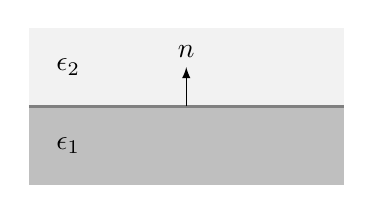
\begin{tikzpicture};
		\fill[gray!50] (0,-1) rectangle (4,0);
		\fill[gray!10] (0,1) rectangle (4,0);
		\draw[thick, gray] (0,0) -- (4,0);
		\draw[-latex] (2,0) -- +(0,0.5) node[above] {$\vect{n}$};
		\node at (0.5,-0.5) {$\epsilon_1$};
		\node at (0.5,0.5) {$\epsilon_2$};
	\end{tikzpicture}
\end{center}

\end{Theory}

%=========================================================
\begin{problem}
    Два однакових точкових заряди (величина заряду $q$) знаходяться на відстані $l$ один від одного в твердому діелектриці з проникністю $\epsilon$. Заряди розташовані в центрах малих сферичних порожнин. Знайдіть силу взаємодії зарядів.
\begin{solution}
	$ F = \frac{q^2}{l^2} \frac{2 + \epsilon}{3\epsilon}.$
\end{solution}
\end{problem}


\subsection*{Визначення сил, що діють на провідники в електростатичному полі}

%=========================================================
\begin{problem}\label{prb:cutted_sphere}%Lim 1039
Металеву сферу із загальним зарядом $q$ розрізали навпіл. Яку силу необхідно прикласти, щоб утримати половини разом? Сферу вважати нескінченно тонкою.
\begin{solution}
	$F = \frac{q^2}{8R^2}$.
\end{solution}
\end{problem}

%=========================================================
\begin{problem}
Як зміниться відповідь в задачі~\ref{prb:cutted_sphere}, якщо в центрі сфери помістити додатково точковий заряд~$q_0$?
\begin{solution}
	$F = \frac{q(q + 2q_0)}{8R^2}$.
\end{solution}
\end{problem}

%=========================================================
\begin{problem}
Нескінченно довга тонка провідна циліндрична оболонка радіусом $ R $ розрізана уздовж осі. Визначити силу відштовхування, що діє на одиницю довжини кожної половини, якщо на одиницю довжини оболонки припадає заряд $ \lambda $.
\begin{solution}
	$F = \frac{\lambda^2}{\pi R}$.
\end{solution}
\end{problem}

%=========================================================
\begin{problem}
Незаряджена металева сфера маси $m$ плаває в діелектричній рідини з проникністю $\epsilon$, занурившись в неї на одну чверть свого об'єму. До якого потенціалу слід зарядити сферу, щоб вона плавала зануреною в неї на половину?
\begin{solution}
	$\phi = \sqrt{\frac{2mg(1+\epsilon)^2}{\pi\epsilon}}$.
\end{solution}
\end{problem}

%=========================================================
\begin{problem}% Миронова V.11
Знайти силу взаємодії двох однакових незаряджених металевих сфер радіусами $R$, вміщених в однорідне електричне поле з напруженістю $E_0$, яке напрямне паралельно лінії, що з'єднує центри сфер. Відстань між центрам сфер дорівнює $l$, причому $l \gg R$.
\begin{solution}
	$F = \frac{6R^6}{l^4} E_0$.
\end{solution}
\end{problem}

%=========================================================
\begin{problem}
З якою силою притягуються пластини плоского конденсатора у вакуумі, заряд якого $q$, а площа пластин $S$?
\begin{solution}
	$F = \frac{2\pi q^2}{S}$.
\end{solution}
\end{problem}

%=========================================================
\begin{problem}
Між обкладками плоского повітряного конденсатора розташована діелектрична пластина товщиною $d_2$ з діелектричною проникністю $\epsilon$, сумарна товщина повітряних зазорів між пластиною та обкладками дорівнює $d_1$. Різниця потенціалів між обкладками дорівнює $V$. Визначити силу притягання між обкладками. Площа всіх пластин дорівнює~$S$.
\begin{solution}
	$ F = \frac{S}{8\pi} \left( \frac{\epsilon V}{ \epsilon d_1 + d_2} \right)^2 $.
\end{solution}
\end{problem}

\subsection*{Визначення сил, що діють на діелектрики в електростатичному полі}

%=========================================================
\begin{problem}
    Відомо, що легкі діелектричні тіла притягуються до наелектризованих тіл. Чому це відбувається? Чи може бути ситуація, коли діелектричні тіла відштовхуватимуться від наелектризованого тіла?
\end{problem}

%=========================================================
\begin{problem}
	Нехай однорідний діелектрик у вигляді витягнутого еліпсоїда з проникністю $\epsilon_2$ знаходиться в середовищі з проникністю $\epsilon_1$. Покажіть, що при вміщенні такого тіла в неоднорідне електричне поле, воно орієнтуватиметься вздовж силових ліній якщо його $\epsilon_2 > \epsilon_1$, і перпендикулярно силовим лініям у випадку, якщо $\epsilon_2 < \epsilon_1$.
\end{problem}

%=========================================================
\begin{problem}
    Для задачі~\ref{prb:half_filled_condensator} знайдіть силу, що діє на одиницю поверхні діелектрика в обох випадках.
	\begin{solution}
		У випадку паралельного заповнення до обкладок:
		\begin{enumerate*}[label=\alph*)]
			\item за постійної напруги
			$\vect{f} = \frac{1}{8\pi}\left( 1+\frac1\epsilon\right) \frac{2\epsilon}{\epsilon + 1} E_0^2 \vect{n}$;
			\item за постійного заряду
			$\vect{f} = \frac{1}{8\pi}\left( 1+\frac1\epsilon\right) E_0^2 \vect{n}$.
		\end{enumerate*}
		У випадку перпендикулярно заповнення до обкладок:
		\begin{enumerate*}[label=\alph*)]
			\item за постійної напруги
			$\vect{f} = \frac{1}{8\pi}\epsilon E_0^2 \vect{n}$;
			\item за постійного заряду
			$\vect{f} = \frac{1}{8\pi} \frac{2\epsilon }{\epsilon + 1} E_0^2 \vect{n}$.
		\end{enumerate*}
		Де $\vect{n}$~-- напрямлений перпендикулярно до поверхні розділу у вакуум.
	\end{solution}
\end{problem}

%=========================================================
\begin{problem}\label{prb:plate_into_condensator}
    З якою силою втягується діелектрична пластина в плоский конденсатор, якщо вона входить в простір між обкладинками на довжину $x$ (рис.~\ref{plate_into_condensator})? Розглянути випадки
	\begin{enumerate*}[label=\alph*)]
		\item заряд на пластинках є постійним і рівним $Q$;
		\item потенціал на пластинках підтримується постійним і рівним $V$.
	\end{enumerate*}
	Відстань між обкладками $d$, довжина обкладок $l$, а ширина $a$. Діелектрична проникність пластини $\epsilon$. Вважати, що $x \gg d$ і $l - x \gg d$. Поясніть сенс цих умов. Порівняйте значення сил в обох випадках, якщо $Q = CV$.
\end{problem}

%---------------------------------------------------------
\begin{figure}[h!]\centering
    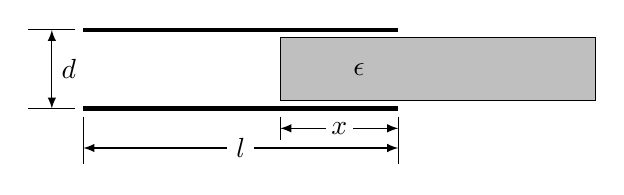
\begin{tikzpicture}
        \draw[ultra thick] (-2,0.5) -- (2,0.5);
		\draw[ultra thick] (-2,-0.5) -- (2,-0.5);
		\fill[gray!50, draw = black] (0.5,-0.4) rectangle (4.5,0.4);
		\node at (1.5,0) {$\epsilon$};
		\draw (0.5, -0.6) -- +(0,-0.3) (2, -0.6) -- +(0,-0.6);
		\draw (-2, -0.6) -- +(0,-0.6);
		\draw[latex-latex] (0.5, -0.75) -- node[fill=white, inner sep=2pt] {$x$} (2, -0.75);
		\draw[latex-latex] (-2, -1) -- node[fill=white] {$l$} (2, -1);
		\draw (-2.1, 0.5) -- (-2.7, 0.5) (-2.1, -0.5) -- (-2.7, -0.5);
		\draw[latex-latex] (-2.4, 0.5) -- node[right] {$d$} (-2.4,-0.5);
    \end{tikzpicture}
\caption{До задачі~\ref{prb:plate_into_condensator}}
\label{plate_into_condensator}
\end{figure}
%---------------------------------------------------------




%=========================================================
\begin{problem}%Батигін 138
Плоский конденсатор занурено в ідеальну рідину з діелектричною проникністю $\epsilon$ і густиною $\rho$ так, що його обкладки розташовані вертикально. Відтань між ними дорівнює $d$, різниця потенціалів $V$. Визначити висоту підняття рідини в конденсаторі.
\begin{solution}
	$h = \frac{\epsilon - 1}{8\pi g \rho} \left(\frac{V}{d} \right)^2$.
\end{solution}
\end{problem}

%=========================================================
\begin{problem}% Миронова V.26
Довгий тонкий циліндричний стрижень з однорідного ізотропного діелектрика з діелектричною проникністю $\epsilon$ знаходиться в однорідному електричному полі з напруженістю $E_0$, що утворює кут $\alpha$ з напрямком осі стрижня. Об'єм стрижня дорівнює $V$. Який зовнішній момент сил слід прикласти, щоб утримати стрижень в даному положенні?
\begin{solution}
	$M = \frac{V}{8\pi} \frac{(\epsilon - 1)^2}{\epsilon + 1} E_0^2\sin2\alpha$.
\end{solution}
\end{problem}

%=========================================================
\begin{problem}\label{prb:ballunderring}
На осі симетрії тонкого кільця радіусом $R$, зарядженого зарядом $q$, на відстані $z$ від його центру розташована діелектрична кулька радіусом $r$ ($r \ll R$) з діелектричною проникністю діелектрика $\epsilon$~(рис.~\ref{ballunderring}). Яка сила діє на кульку з боку електричного поля?
\begin{solution}
	$\vect F = q^2\frac{\epsilon - 1}{\epsilon + 2}r^3 \frac{z(R^2 - 2z^2)}{(R^2 + z^2)^4} \vect k.$
\end{solution}
\end{problem}
%---------------------------------------------------------
\begin{figure}[h!]\centering
	\begin{tikzpicture}
		\draw[thick, red] (0,0) ellipse (4 and 1);
		\draw[-latex'] (0,0) -- node[below] {$R$} (170:3.3);
		\draw[dash dot] (0,0) -- node [left] {$z$} (0,3);
		\draw[ball color=gray!50] (0,3.3) circle (0.3) node {$\epsilon$};
	\end{tikzpicture}
	\caption{До задачі~\ref{prb:ballunderring}}
	\label{ballunderring}
\end{figure}
%---------------------------------------------------------

%=========================================================
\begin{problem}% Миронова V.25
Для умов задачі~\ref{prb:ballunderring} визначити, у яких точках $z$ на осі кільця сила, що діє на кульку буде
\begin{enumerate*}[label=\alph*)]
	\item мінімальною,
	\item максимальною,
	\item дорівнюватиме нулю?
\end{enumerate*}
\begin{solution}
	\begin{enumerate*}[label=\alph*)]
		\item $F \approx \frac{0.13r^3}{3R^5} (\epsilon - 1) Q^2$, при $z = 0.286 R$;
		\item $F \approx - \frac{0.13r^3}{3R^5} (\epsilon - 1) Q^2$, при $z = 1.104 R$;
		\item При $z = 0$, положення нестійкої рівноваги, та при $z = \nfrac{R}{\sqrt2}$, положення стійкої рівноваги.
	\end{enumerate*}
\end{solution}
\end{problem}

%=========================================================
\begin{problem}%Журнал Квант, №5, стор 13
    Два точкові заряди $q_1$ та $q_2$ знаходяться на відстані $r$ один від одного в центрах малих сферичних порожнин в твердому діелектрику з проникністю $\epsilon$. Знайдіть сили, що діють на заряди.
\begin{solution}
	$F_1 = F_2 = \frac{3\epsilon}{2\epsilon + 1}\frac{q_1q_2}{r^2}$.
\end{solution}
\end{problem}


\Closesolutionfile{answer}

